%%%  کلاس AUTthesis، نسخه آبان 1397
%%%   دانشگاه صنعتی امیرکبیر                 http://www.aut.ac.ir
%%%  تالار گفتگوی پارسی‌لاتک،       http://forum.parsilatex.com
%%%   آپدیت شده در آبان 95
%%%   پشتیبانی و راهنمایی          badali_farhad@yahoo.com
%%%
%%%   بازبینی و اصلاح شده در آبان ماه 1397
%%%  Tested via TeXstudio in TeXlive 2014-2018.
%%%

%-----------------------------------------------------------------------------------------------------
%        روش اجرا.: 2 بار F1 ، 2 بار  F11(به منظور تولید مراجع) ، دوبار Ctrl+Alt+I (به منظور تولید نمایه) و دو بار F1 -------> مشاهده Pdf
%%%%%%%%%%%%%%%%%%%%%%%%%%%%%%%%%%%%%%%%%%%%%%%%%%%%%%
%   TeXstudio as your IDE
%%  برای compile در TeXstudio تنها کافی است منوی Options->Configure TeXstudio را زده و در پنجره Configure TeXstudio در بخش Build گزینه Default Compiler را به XeLaTeX تغییر دهید. سند شما به راحتی compile خواهد شد.
%   F1 & F5 : Build & view
%   F6      : Compile
%   F7      : View
%   --------------
%%%%%%%%%%%%%%%%%%%%%%%%%%%%%%%%%%%%%%%%%%%%%%%%%%%%%%
%        اگر قصد نوشتن رساله دکتری را دارید، در خط زیر به جای msc،
%      کلمه phd را قرار دهید. کلیه تنظیمات لازم، به طور خودکار، اعمال می‌شود.
%%% !TEX TS-program = XeLaTeX
\documentclass[oneside,bsc,12pt]{AUTthesis}
%       فایل commands.tex را حتماً به دقت مطالعه کنید؛ چون دستورات مربوط به فراخوانی بسته زی‌پرشین 
%       و دیگر بسته‌ها و ... در این فایل قرار دارد و بهتر است که با نحوه استفاده از آنها آشنا شوید. توجه شود برای نسخه نهایی پایان‌نامه حتماً hyperref را 
%        غیرفعال کنید.


% در این فایل، دستورها و تنظیمات مورد نیاز، آورده شده است.
%-------------------------------------------------------------------------------------------------------------------
% در ورژن جدید زی‌پرشین برای تایپ متن‌های ریاضی، این سه بسته، حتماً باید فراخوانی شود.
\usepackage{amsthm,amssymb,amsmath,amsfonts}
% بسته‌ای برای تنطیم حاشیه‌های بالا، پایین، چپ و راست صفحه
\usepackage[top=30mm, bottom=30mm, left=25mm, right=30mm]{geometry}
% بسته‌‌ای برای ظاهر شدن شکل‌ها و تصاویر متن
\usepackage{graphicx}
\usepackage{color}
%بسته‌ای برای تنظیم فاصله عمودی خط‌های متن
\usepackage{setspace}
\usepackage{titletoc}
\usepackage{tocloft}
%با فعال کردن بسته زیر فوت‌نوت‌ها در هر صفحه ریست می‌شوند. حالت پیش‌فرض آن ریست شدن در هر فصل می‌باشد.
%\usepackage[perpage]{footmisc}
\usepackage{enumitem}
%\usepackage{titlesec}
% بسته‌ و دستوراتی برای ایجاد لینک‌های رنگی با امکان جهش
\usepackage[pagebackref=false,colorlinks,linkcolor=blue,citecolor=red]{hyperref}
\usepackage[nameinlink]{cleveref}%capitalize,,noabbrev
 \AtBeginDocument{%
    \crefname{equation}{برابری}{equations}%
    \crefname{chapter}{فصل}{chapters}%
    \crefname{section}{بخش}{sections}%
    \crefname{appendix}{پیوست}{appendices}%
    \crefname{enumi}{مورد}{items}%
    \crefname{footnote}{زیرنویس}{footnotes}%
    \crefname{figure}{شکل}{figures}%
    \crefname{table}{جدول}{tables}%
    \crefname{theorem}{قضیه}{theorems}%
    \crefname{lemma}{لم}{lemmas}%
    \crefname{corollary}{نتیجه}{corollaries}%
    \crefname{proposition}{گزاره}{propositions}%
    \crefname{definition}{تعریف}{definitions}%
    \crefname{result}{نتیجه}{results}%
    \crefname{example}{مثال}{examples}%
    \crefname{remark}{نکته}{remarks}%
    \crefname{note}{یادداشت}{notes}%
}
% چنانچه قصد پرینت گرفتن نوشته خود را دارید، خط بالا را غیرفعال و  از دستور زیر استفاده کنید چون در صورت استفاده از دستور زیر‌‌، 
% لینک‌ها به رنگ سیاه ظاهر خواهند شد که برای پرینت گرفتن، مناسب‌تر است
%\usepackage[pagebackref=false]{hyperref}
% بسته‌ لازم برای تنظیم سربرگ‌ها
\usepackage{fancyhdr}
% بسته‌ای برای ظاهر شدن «مراجع»  در فهرست مطالب
\usepackage[nottoc]{tocbibind}
% دستورات مربوط به ایجاد نمایه

\usepackage{listings}

\usepackage{makeidx,multicol}
\setlength{\columnsep}{1.5cm}

%%%%%%%%%%%%%%%%%%%%%%%%%%
\usepackage{verbatim}
\makeindex
\usepackage{sectsty}
% فراخوانی بسته زی‌پرشین و تعریف قلم فارسی و انگلیسی
\usepackage{xepersian}%[extrafootnotefeatures]
\SepMark{-}
%حتماً از تک لایو 2014 استفاده کنید.
\settextfont[Scale=1.2]{B-NAZANIN.TTF}
\setlatintextfont{times.ttf}
\renewcommand{\labelitemi}{$\bullet$}
%%%%%%%%%%%%%%%%%%%%%%%%%%
% چنانچه می‌خواهید اعداد در فرمول‌ها، انگلیسی باشد، خط زیر را غیرفعال کنید.
%در غیر اینصورت حتماً فونت PGaramond را نصب کنید.
%\setdigitfont[Scale=1.1]{PGaramond.ttf}%%Yas
%%%%%%%%%%%%%%%%%%%%%%%%%%
% تعریف قلم‌های فارسی اضافی برای استفاده در بعضی از قسمت‌های متن
\defpersianfont\nastaliq[Scale=2]{IranNastaliq.ttf}
\defpersianfont\chapternumber[Scale=3]{B-NAZANIN.TTF}
%\chapterfont{\centering}%
%%%%%%%%%%%%%%%%%%%%%%%%%%
% دستوری برای تغییر نام کلمه «اثبات» به «برهان»
\renewcommand\proofname{\textbf{برهان}}

% دستوری برای تغییر نام کلمه «کتاب‌نامه» به «منابع و مراجع«
\renewcommand{\bibname}{منابع و مراجع}


% Headings for every page of ToC, LoF and Lot
\setlength{\cftbeforetoctitleskip}{-1.2em}
\setlength{\cftbeforelottitleskip}{-1.2em}
\setlength{\cftbeforeloftitleskip}{-1.2em}
\setlength{\cftaftertoctitleskip}{-1em}
\setlength{\cftafterlottitleskip}{-1em}
\setlength{\cftafterloftitleskip}{-1em}
%%\makeatletter
%%%%\renewcommand{\l@chapter}{\@dottedtocline{1}{1em\bfseries}{1em}}
%%%%\renewcommand{\l@section}{\@dottedtocline{2}{2em}{2em}}
%%%%\renewcommand{\l@subsection}{\@dottedtocline{3}{3em}{3em}}
%%%%\renewcommand{\l@subsubsection}{\@dottedtocline{4}{4em}{4em}}
%%%%\makeatother


\newcommand\tocheading{\par عنوان\hfill صفحه \par}
\newcommand\lofheading{\hspace*{.5cm}\figurename\hfill صفحه \par}
\newcommand\lotheading{\hspace*{.5cm}\tablename\hfill صفحه \par}

\renewcommand{\cftchapleader}{\cftdotfill{\cftdotsep}}
\renewcommand{\cfttoctitlefont}{\hspace*{\fill}\LARGE\bfseries}%\Large
\renewcommand{\cftaftertoctitle}{\hspace*{\fill}}
\renewcommand{\cftlottitlefont}{\hspace*{\fill}\LARGE\bfseries}%\Large
\renewcommand{\cftafterlottitle}{\hspace*{\fill}}
\renewcommand{\cftloftitlefont}{\hspace*{\fill}\LARGE\bfseries}
\renewcommand{\cftafterloftitle}{\hspace*{\fill}}

%%%%%%%%%%%%%%%%%%%%%%%%%%
% تعریف و نحوه ظاهر شدن عنوان قضیه‌ها، تعریف‌ها، مثال‌ها و ...
%برای شماره گذاری سه تایی قضیه ها
\theoremstyle{definition}
\newtheorem{definition}{تعریف}[section]
\newtheorem{remark}[definition]{نکته}
\newtheorem{note}[definition]{یادداشت}
\newtheorem{example}[definition]{نمونه}
\newtheorem{question}[definition]{سوال}
\newtheorem{remember}[definition]{یاداوری}
\theoremstyle{theorem}
\newtheorem{theorem}[definition]{قضیه}
\newtheorem{lemma}[definition]{لم}
\newtheorem{proposition}[definition]{گزاره}
\newtheorem{corollary}[definition]{نتیجه}
%%%%%%%%%%%%%%%%%%%%%%%%
%%%%%%%%%%%%%%%%%%%
%%% برای شماره گذاری چهارتایی قضیه ها و ...
%%\newtheorem{definition1}[subsubsection]{تعریف}
%%\newtheorem{theorem1}[subsubsection]{قضیه}
%%\newtheorem{lemma1}[subsubsection]{لم}
%%\newtheorem{proposition1}[subsubsection]{گزاره}
%%\newtheorem{corollary1}[subsubsection]{نتیجه}
%%\newtheorem{remark1}[subsubsection]{نکته}
%%\newtheorem{example1}[subsubsection]{مثال}
%%\newtheorem{question1}[subsubsection]{سوال}

%%%%%%%%%%%%%%%%%%%%%%%%%%%%

% دستورهایی برای سفارشی کردن صفحات اول فصل‌ها
\makeatletter
\newcommand\mycustomraggedright{%
 \if@RTL\raggedleft%
 \else\raggedright%
 \fi}
\def\@makechapterhead#1{%
\thispagestyle{style1}
\vspace*{20\p@}%
{\parindent \z@ \mycustomraggedright
\ifnum \c@secnumdepth >\m@ne
\if@mainmatter

\bfseries{\Huge \@chapapp}\small\space {\chapternumber\thechapter}
\par\nobreak
\vskip 0\p@
\fi
\fi
\interlinepenalty\@M 
\Huge \bfseries #1\par\nobreak
\vskip 120\p@

}

%\thispagestyle{empty}
\newpage}
\bidi@patchcmd{\@makechapterhead}{\thechapter}{\tartibi{chapter}}{}{}
\bidi@patchcmd{\chaptermark}{\thechapter}{\tartibi{chapter}}{}{}
\makeatother

\pagestyle{fancy}
\renewcommand{\chaptermark}[1]{\markboth{\chaptername~\tartibi{chapter}: #1}{}}

\fancypagestyle{style1}{
\fancyhf{} 
\fancyfoot[c]{\thepage}
\fancyhead[R]{\leftmark}%
\renewcommand{\headrulewidth}{1.2pt}
}


\fancypagestyle{style2}{
\fancyhf{}
\fancyhead[R]{چکیده}
\fancyfoot[C]{\thepage{}}
\renewcommand{\headrulewidth}{1.2pt}
}

% \fancypagestyle{style3}{%
%   \fancyhf{}%
%   \fancyhead[R]{فهرست نمادها}
%   \fancyfoot[C]{\thepage}%
%   \renewcommand{\headrulewidth}{1.2pt}%
% }

\fancypagestyle{style4}{%
  \fancyhf{}%
  \fancyhead[R]{فهرست جداول}
  \fancyfoot[C]{\thepage}%
  \renewcommand{\headrulewidth}{1.2pt}%
}

\fancypagestyle{style5}{%
  \fancyhf{}%
  \fancyhead[R]{فهرست اشکال}
  \fancyfoot[C]{\thepage}%
  \renewcommand{\headrulewidth}{1.2pt}%
}

\fancypagestyle{style6}{%
  \fancyhf{}%
  \fancyhead[R]{فهرست مطالب}
  \fancyfoot[C]{\thepage}%
  \renewcommand{\headrulewidth}{1.2pt}%
}

\fancypagestyle{style7}{%
  \fancyhf{}%
  \fancyhead[R]{نمایه}
  \fancyfoot[C]{\thepage}%
  \renewcommand{\headrulewidth}{1.2pt}%
}

\fancypagestyle{style8}{%
  \fancyhf{}%
  \fancyhead[R]{منابع و مراجع}
  \fancyfoot[C]{\thepage}%
  \renewcommand{\headrulewidth}{1.2pt}%
}
\fancypagestyle{style9}{%
  \fancyhf{}%
  \fancyhead[R]{واژه‌نامه‌ی فارسی به انگلیسی}
  \fancyfoot[C]{\thepage}%
  \renewcommand{\headrulewidth}{1.2pt}%
}
%


%دستور حذف نام لیست تصاویر و لیست جداول از فهرست مطالب
\newcommand*{\BeginNoToc}{%
  \addtocontents{toc}{%
    \edef\protect\SavedTocDepth{\protect\the\protect\value{tocdepth}}%
  }%
  \addtocontents{toc}{%
    \protect\setcounter{tocdepth}{-10}%
  }%
}
\newcommand*{\EndNoToc}{%
  \addtocontents{toc}{%
    \protect\setcounter{tocdepth}{\protect\SavedTocDepth}%
  }%
}
\newcounter{savepage}
\renewcommand{\listfigurename}{فهرست اشکال}
\renewcommand{\listtablename}{فهرست جداول}
%\renewcommand\cftsecleader{\cftdotfill{\cftdotsep}}
%%%%%%%%%%%%%%%%%%%%%%%%%%%%%
%%%%%%%%%%%%%%%%%%%%%%%%%%%%

\begin{document}
\baselineskip=.75cm
\linespread{1.75}
%% -!TEX root = AUTthesis.tex
% در این فایل، عنوان پایان‌نامه، مشخصات خود، متن تقدیمی‌، ستایش، سپاس‌گزاری و چکیده پایان‌نامه را به فارسی، وارد کنید.
% توجه داشته باشید که جدول حاوی مشخصات پروژه/پایان‌نامه/رساله و همچنین، مشخصات داخل آن، به طور خودکار، درج می‌شود.
%%%%%%%%%%%%%%%%%%%%%%%%%%%%%%%%%%%%
% دانشکده، آموزشکده و یا پژوهشکده  خود را وارد کنید
\faculty{دانشکده مهندسی کامپیوتر}
% گرایش و گروه آموزشی خود را وارد کنید
 \department{}
% عنوان پایان‌نامه را وارد کنید
% \fatitle{
% 	درس داده‌کاوی
% }
% نام استاد(ان) راهنما را وارد کنید
% \firstsupervisor{دکتر مریم امیر مزلقانی}
%\secondsupervisor{استاد راهنمای دوم}
% نام استاد(دان) مشاور را وارد کنید. چنانچه استاد مشاور ندارید، دستور پایین را غیرفعال کنید.
% \firstadvisor{دکتر حامد فربه}
%\secondadvisor{استاد مشاور دوم}
% نام نویسنده را وارد کنید
% \name{امیرحسین پاشایی‌هیر، حیدر فهمی، مهدی قیاسی }
% نام خانوادگی نویسنده را وارد کنید
\surname{}
%%%%%%%%%%%%%%%%%%%%%%%%%%%%%%%%%%
% \thesisdate{زمستان ۱۴۰۰}

% چکیده پایان‌نامه را وارد کنید
\fa-abstract{
در این گزارش به بررسی روشی به نام تی اس ان ای می‌پردازیم که هدف آن مصور سازی داده‌هایی با ابعاد بالا می‌باشد که این هدف را با نگاشت کردن هر داده به یک نقطه در فضای دو یا سه بعدی انجام می‌دهد. این روش یک نسخه از روش تعبیه همسایه تصادفی (یا اس ان ای) می‌باشد که بهینه کردن آن بسیار راحت‌تر بوده و با کم کردن گرایش نقاط متراکم به مرکز، خروجی به مراتب بهتری تحویل می‌دهد. تی اس ان ای از روش‌های موجود، عملکرد بهتری در ارائه انواع ساختارهای داده کلی در قالب یک نگاشت، ارائه می‌دهد. این عملکرد بخصوص برای داده‌هایی که ابعاد بالایی دارند اما در اصل به روی چند منحی با ابعادی پایین قرار داده شده‌اند بسیار مهم می‌شود. برای مصور سازی ساختار داده‌های با ابعاد بالا، بررسی می‌کنیم که تی اس ان ای چگونه با استفاده از قدم زدن اتفاقی به روی گراف همسایگی می‌تواند ساختار داده‌ها را خلاصه کند و آن‌ها را مصور سازی کند، ما همچنین به مقایسه‌ی عملکرد روش تی اس ان ای نسبت به تعداد زیادی از روش‌ها مانند نگاشت سامون، ایزومپ و تعبیه خطی محلی می‌پردازیم و در نتیجه می‌بینم که تی اس ان ای، مصور سازی به مراتب بهتری نسبت به بقیه روش‌ها بر روی تمام مجموعه داده‌ها ارائه داده است.
}


% کلمات کلیدی پایان‌نامه را وارد کنید
\keywords{مصورسازی، کاهش بعد، الگوریتم‌های تعبیه سازی، مقیاس چندبعدی}



\AUTtitle
%%%%%%%%%%%%%%%%%%%%%%%%%%%%%%%%%%
% \vspace*{7cm}
% \thispagestyle{empty}
% \begin{center}
% 
\includegraphics[height=5cm,width=12cm]{besm}
% \end{center}
% تاییدیه دفاع
% \newpage
\thispagestyle{empty}
%\fontsize{18pt}{19pt}\selectfont

\section*{صفحه فرم ارزیابی و تصویب پایان نامه- فرم تأیید اعضاء كميته دفاع}

\fontsize{12pt}{14pt}\selectfont
%\renewcommand{\baselinestretch}{1.5}
\vspace*{1cm}
   در این صفحه فرم دفاع یا تایید و تصویب پایان نامه موسوم به فرم کمیته دفاع- موجود در پرونده آموزشی- را قرار دهید.
\vspace*{1cm}


\subsection*{نکات مهم:}
 
\begin{itemize}
\item
	نگارش پایان نامه/رساله باید به
	{\color{red}
		زبان فارسی
	}
	و بر اساس آخرین نسخه دستورالعمل و راهنمای تدوین پایان نامه های دانشگاه صنعتی امیرکبیر باشد.(دستورالعمل و راهنمای حاضر)
\item رنگ جلد پایان نامه/رساله چاپي كارشناسي، كارشناسي ارشد و دكترا  بايد به ترتيب مشكي، طوسي و سفيد رنگ باشد.  
\item چاپ و صحافی پایان نامه/رساله بصورت
{\color{red}
	پشت و رو(دورو)
}
بلامانع است و انجام آن توصيه مي شود. 
\end{itemize}
%%%%%%%%%%%%%%%%%%%%%%%%%%%%%%%%%%%%%%%%%%%%%%%%%%%%%%%%%%%%%%%%%%%%%%%%%%%%%%%%%%%%%%%%%%%%%%%%%%
%%%%%%%%%%%%%%%%%%%%%%%%%%%%%%%%%%%%%%%%%%%%%%%%%%%%%%%%%%%%%%%%%%%%%%%%%%%%%%%%%%%%%%%%%%%%%%%%%%
\newpage
\thispagestyle{empty}
\begin{picture}(50,50)
  \put(17,0){
\includegraphics[scale=1.1]{fa-logo}}
  \put(4.5,-13){\footnotesize{دانشگاه صنعتی امیرکبیر}}
  \put(10.5,-27){\footnotesize{(پلی‌تکنیک تهران)}}
  \put(170,30){\bf{به نام خدا}}
  \put(140,-5){\Large\bf{تعهدنامه اصالت اثر}}
  \put(310,0){تاریخ: \datethesis}
\end{picture}

\vspace*{2.5cm}

اينجانب {\bf{\fname\lname}} متعهد می‌شوم که مطالب مندرج در این پایان‌نامه حاصل کار پژوهشی اینجانب تحت نظارت و راهنمایی اساتید دانشگاه صنعتی امیرکبیر بوده و به دستاوردهای دیگران که در این پژوهش از آنها استفاده شده است مطابق مقررات و روال متعارف ارجاع و در فهرست منابع و مآخذ ذکر گردیده است. این پایان‌نامه قبلاً برای احراز هیچ مدرک هم‌سطح یا بالاتر ارائه نگردیده است.

در صورت اثبات تخلف در هر زمان، مدرک تحصیلی صادر شده توسط دانشگاه از درجه اعتبار ساقط بوده و دانشگاه حق پیگیری قانونی خواهد داشت.


کلیه نتایج و حقوق حاصل از این پایان‌نامه متعلق به دانشگاه صنعتی امیرکبیر می‌باشد. هرگونه استفاده از نتایج علمی و عملی، واگذاری اطلاعات به دیگران یا چاپ و تکثیر، نسخه‌برداری، ترجمه و اقتباس از این پایان نامه بدون موافقت کتبی دانشگاه صنعتی امیرکبیر ممنوع است. 
نقل مطالب با ذکر مآخذ بلامانع است.\\
\vspace{2.5cm}


{\centerline {\bf{\fname\lname}}}
\vspace*{.2cm}
{\centerline{امضا}}
%%%%%%%%%%%%%%%%%%%%%%%%%%%%%%%%%
% چنانچه مایل به چاپ صفحات «تقدیم»، «نیایش» و «سپاس‌گزاری» در خروجی نیستید، خط‌های زیر را با گذاشتن ٪  در ابتدای آنها غیرفعال کنید.
% پایان‌نامه خود را تقدیم کنید
% نیایش خود را در فایل زیر بنویسید.
%\begin{acknowledgementpage}

\vspace{1.5cm}

{\nastaliq
{
تقدیم به علی یونسی و امیرحسین مرادی که در بندند.
}}\end{acknowledgementpage}
\newpage
% سپاسگزاری را در فایل زیر بنویسید.
% %%%%%%%%%%%%%%%%%%%%%%%%%%%%%%%%%%%%
\newpage\thispagestyle{empty}
% سپاس‌گزاری
{\nastaliq
سپاس‌گزاری
}
\\[2cm]

وظیفه خود می‌دانیم که مراتب امتنان خود را نسبت به استادمان در درس داده‌کاوی، دکتر مریم امیر مزلقانی که ما را یاری نموده‌اند، اعلام بداریم.














% با استفاده از دستور زیر، امضای شما، به طور خودکار، درج می‌شود.
\signature








%%%%%%%%%%%%%%%%%%%%%%%%%%%%%%%%%%%%%%%%%
%%%%%%%%%%%%%%%%%%%%%%%%%%%%%%%%%کدهای زیر را تغییر ندهید.
\newpage\clearpage

\pagestyle{style2}

\vspace*{-1cm}
\section*{\centering چکیده}
%\addcontentsline{toc}{chapter}{چکیده}
\vspace*{.5cm}
\ffa-abstract
\vspace*{2cm}


{\noindent\large\textbf{واژه‌های کلیدی:}}\par
\vspace*{.5cm}
\fkeywords
% دستور زیر برای شماره گذاری صفحات قبل از فصل اول با حروف ابجد است.
\pagenumbering{alph}
%-----------------------------------------------------------------------------
% فایل زیر دستورات مربوط به نمایش صفحات فهرست مطالب- فهرست اشکال و جداول است.
% %{\pagestyle{style2}
%\tableofcontents}\newpage
%
%\listoffigures
\cleardoublepage
\pagestyle{style6}
\tableofcontents
\pagestyle{style6}
\cleardoublepage
%اگر لیست تصاویر و لیست جداول ندارید ، کدهای زیر را با گذاشتن % در ابتدای آنها، غیرفعال کنید.
\BeginNoToc
%============
\addtocontents{lof}{\lofheading}% add heading to the first page in LoF
\pagestyle{style5}
\listoffigures
\thispagestyle{style5}
\cleardoublepage
%============
% \addtocontents{lot}{\lotheading}% add heading to the first page in LoT
% \thispagestyle{style4}
% \listoftables
% \thispagestyle{style4}
%============
%\cleardoublepage
%
\cleardoublepage
\setcounter{savepage}{\arabic{page}}
\mainmatter
\addtocontents{toc}{\tocheading}% add heading to the first page in ToC, after frontmatter entries
\EndNoToc
% در صورت تمایل می‌توانید با فعال کردن دستور بالا، لیست تصاویر را به  پایان‌نامه خود اضافه کنید.
%-------------------------------------------------------------------------symbols(فهرست نمادها)
% وجود لیست نمادها الزامیست.(لطفاً نمادهای خود را جایگذین نمادهای پیش‌فرض کنید.)
% %%%%%%%%%%%%%

\pagenumbering{alph}
\setcounter{page}{\thesavepage}
%\setcounter{page}{6}
\vspace*{1cm}

\pagestyle{style3}
\thispagestyle{style3}
\newpage
%\pagestyle{style1}
%%%%%%%%%%%%%%%%%%%%%%%%%%%%%%%%%%%%


\pagenumbering{arabic}
\pagestyle{style1}
%--------------------------------------------------------------------------chapters(فصل ها)
% \chapter{مقدمه}
% {مصور سازی}\LTRfootnote{Visualization}
%  داده‌های با ابعاد بالا مسئله‌ی مهمی در بسیاری از دامنه‌ها می‌باشد. این مسئله با بازه‌ی بزرگی از ابعاد (از سی بعد برای داده‌های پزشکی تا ده‌ها هزار بعد برای داده‌های سند‌ها) درگیر است.
% \\
% در دهه‌ی اخیر راه‌حل‌های متنوعی برای این مسئله ارائه شده است
% \cite{lee2007nonlinear}
%  که می‌توان به روش‌های شمایل نگاری، روش‌های براساس
% {پیکسل}\LTRfootnote{Pixel}
% و روش‌هایی که ابعاد را به صورت رئوس گراف نشان می‌دهند اشاره کرد.
% \\
% اکثر این روش‌ها ابزاری ارائه می‌دهند که داده‌ها را بتوان به صورت دو بعدی نمایش داد و تحلیل را به مشاهده انسانی واگذار می‌کنند.
% این موضوع باعث می‌شود که کاربرد این روش‌ها در دنیای واقعی برای داده‌هایی که ده‌ها هزار بعد دارند کم شود.
% \\
% برخلاف روش‌های بالا، روش‌های کاهش بعد سعی می‌کنند داده‌های با ابعاد بالا را به داده‌های دو یا سه بعدی خلاصه کنند.
% \\
% روش‌های خطی و سنتی‌ای مانند
% {تجزیه و تحلیل اجزای اصلی یا پی ‌سی‌ ای}\LTRfootnote{PCA}
% یا 
% {مقایسه چند بعدی کلاسیک یا ام دی اس}\LTRfootnote{MDS}
% روش‌هایی هستند که سعی دارند داده‌های غیرمشابه را پس از نگاشت تا جای ممکن از هم دور نگه دارند. در روش‌های غیرخطی سعی می‌شود که داده‌هایی که در توصیف اصلی خود به همدیگر نزدیک هستند،‌ پس از نگاشت و خلاصه شدن نیز باز هم به همدیگر نزدیک بمانند،‌ که پیاده‌سازی این مهم توسط روش‌های خطی امکان پذیر نمی‌باشد.
% \\
% روش‌های غیرخطی زیادی برای کاهش بعد ارائه شده است که سعی دارند ساختار محلی داده را نگه دارند. از این روش‌ها می‌توان به
% نگاشت سامون،
% {تحلیل و تجزیه اجزای منحنی یا سی سی ای}\LTRfootnote{CCA}
% ،
% {تعبیه همسایه تصادفی یا اس ان ای}\LTRfootnote{SNE}
% \cite{hinton2002stochastic}
% ،
% {حداکثر واریانس آشکار یا ام وی یو}\LTRfootnote{MVU}
% ،
% {تعبیه خطی محلی یا ال ال ای}\LTRfootnote{LLE}
% و
% {نگاشت ویژه لاپلاس}\LTRfootnote{Laplacian Eigenmaps}
% اشاره کرد.
% با اینکه روش‌های بر داده‌های مصنوعی با ابعاد بالا بسیار خوب عمل می‌کنند اما در مصور سازی داده‌های با ابعاد بالا، نمی‌توانند عملکرد مناسبی داشته باشند.
% اکثر این روش‌ها نمی‌توانند ساختار عمومی و محلی داده‌ها را در یک نگاشت به خوبی مصور کنند.
% برای مثال، یک مدل ام وی یو با نظارت متوسط نمی‌تواند رقم‌های با دست نوشته را به خوشه‌های طبیعی هر رقم نگاشت کند و رقم‌ها را از هم جدا کند.
% \\
% در این گزارش ما به بررسی روشی می‌پردازیم که داده‌های با ابعاد بالا را به ماتریس شباهت داده‌ها تبدیل می‌کند و سپس با روشی به نام
% {تی اس ان ای}\LTRfootnote{t-SNE}
% \cite{van2008visualizing}
% \cite{rauber2016visualizing}
% این ماتریس به دست آمده را مصور سازی می‌کند.
% \\
% روش تی اس ان ای توانایی نمایش دادن اکثر ساختار محلی داده‌ها را داشته و در کنار آن ساختار عمومی داده‌ها مانند خوشه‌های موجود در داده‌ها را نیز نمایش می‌دهد.
% \\
% در این گزارش ما عملکر تی اس ان ای را با مقایسه کردن آن با هفت روش بیان شده بر روی پنج مجموعه داده‌ی بدست آمده از دامنه‌های مختلف بررسی خواهیم کرد، نتایج نشان می‌دهد که این روش در اکثر دامنه‌ها نسبت به بقیه روش‌ها دارای برتری می‌باشد.
% \\
% در فصل بعدی اس ان ای را معرفی می‌کنیم که مفاهیم آن پایه تی اس ان ای می‌باشد، سپس در فصل بعدی آن تی اس ان ای را معرفی می‌کنیم که دو تفاوت اساسی با اس ان ای دارد، در فصل بعد آن شرایط آزمایش و نتایج آزمایش‌ها را بیان کرده و در فصل بعد آن نشان می‌دهیم که تی اس ان ای چطور می‌تواند تغییر پیدا کند به شکلی که داده‌هایی که ابعاد‌ آن‌ها بسیاری بیشتر از ده هزار بعد است را نمایش دهد و در فصل بعد آن نتایج آزمایش‌ها با دقت بیشتری بررسی می‌شود، در فصل آخر نیز جمع بندی انجام می‌شود.
% \chapter{
% 	۱)بررسی انواع مدل‌های ارائه شده برای دیتابیس‌ها و مزایا و معایب آن‌ها نسبت به مدل رابطه‌ای
% }



\newenvironment{eng}{\begin{LTRbibitems}\resetlatinfont{#1}\end{LTRbibitems}}

\section*{\centering سوال اول
}



می‌دانیم که عملگر
$select$
یک عملگر
$basic$
است.


عملگر
$intersection$
دو عملگر
$select$
را با یکدیگر ترکیب می‌کند، امام تنها سطرهایی را بازمی‌گرداند که در 
$select$
 اول موجود هستند و سطرهایی دقیقا مشابهِ آن‌ها، در
$select$
اول نیز موجود است.


\section*{\centering سوال دوم
}

کوئری اول را بررسی می‌کنیم.
این کوئری، حاصلِ ضربِ کارتزین نتیجه‌ی دو کوئریِ زیر است:




    
% \eng{SELECT A FROM R WHERE B = 7}

\begin{LTRbibitems}\resetlatinfont{SELECT A FROM R WHERE B = 1}\end{LTRbibitems}

\begin{LTRbibitems}\resetlatinfont{SELECT A FROM S WHERE B = 1}\end{LTRbibitems}

% $ SELECT A FROM R WHERE B = 1 $

% $ SELECT C FROM S WHERE B = 1 $

یعنی ابتدا از هر دو جدول، سطرهایی را که مقدار ستون
$B$
مساوی ۱ است، انتخاب می‌کنیم و سپس آن‌ها را با هم ضرب می‌کنیم.
اگر در جدول
$R$
برای مثال، ۲۰ سطر وجود داشته باشد، که از میان این ۲۰ سطر، ۴ سطر باشد که مقدار ستون
$B$
مساوی ۱ است، و در جدول
$S$
۳ سطر باشد که مقدار ستون
$B$
مساوی ۱ است، این کوئری، ۱۲ سطر را باز می‌گرداند.

حال کوئری دوم را بررسی می‌کنیم.
در این کوئری، ابتدا ضرب کارتزین بین نتیجه‌ی این دو کوئری انجام می‌شود:


\begin{LTRbibitems}\resetlatinfont{SELECT A FROM R}\end{LTRbibitems}

\begin{LTRbibitems}\resetlatinfont{SELECT * FROM S WHERE B = 1}\end{LTRbibitems}

یعنی ابتدا از جدول
$R$
همه‌ی سطرها را انتخاب می‌کنیم و سپس از جدول
$S$
سطرهایی را که مقدار ستون
$B$
مساوی ۱ است، انتخاب می‌کنیم.
اگر در جدول
$R$
۴ سطر باشد و در جدول
$S$
۳ سطر باشد، این کوئری، ۱۲ سطر را باز می‌گرداند.

در نهایت، یک  عملگر
$Project$
هم روی نتیجه اعمال شده که ستون‌های
$A$
و
$C$
را بازمی‌گرداند.

بر اساس فرضی که در بخش قبلی مطرح کردیم،‌ در جدول
$R$
۲۰ سطر وجود داشت.
همچنین در جدول
$S$
۳ سطر وجود داشت که مقدار ستون
$B$
مساوی ۱ باشد.
در نتیجه، از ضرب کارتزین این دو، ۶۰ سطر به دست می‌آید.
در نهایت، ستون‌های   
$A$
و
$C$
از این ۶۰ سطر را داریم.
در حالی که در کوئری قبلی، تنها ستون 
$A$
از ۱۲ سطر را داشتیم.
واضح است که این دو کوئری نتایج متفاوتی را بازمی‌گردانند.


حال سومین کوئری را بررسی می‌کنیم.


در این کوئری ابتدا سطرهایی از جدول
$S$
انتخاب شده‌اند که در آن‌ها مقدار ستون
$B$
مساوی ۱ است.


سپس بین حاصل و کل جدول
$R$
عملگر
$Natural Join$
اعمال می‌شود.
این عملگر، ابتدا ستون‌های مشترک را پیدا می‌کند و سپس سطرهایی را از جدول
$R$
انتخاب می‌کند که مقدار ستون‌های مشترک با سطرهای انتخاب شده از جدول
$S$
مساوی باشد.
در این کوئری، ستون مشترک
$B$
است، پس مقادیری بازگردانده می‌شوند که در آن‌ها مقدار
$B$
در هر دو جدول مساوی ۱ باشد.
در نتهایت هم یک 
$Project$
روی نتیجه اعمال می‌شود که ستون‌های
$A$
و
$C$
را باز می‌گرداند.

با فرض‌هایی که در بخش اول در نظر گرفتیم، این کوئری را نیز بررسی می‌کنیم.
از اولین کوئری، تعداد ۳ سطر بازمی‌گردد.

هنگامی که روی این ۳ سطر و کل جدول
$R$
عملگر 
$Natural Join$
اعمال می‌شود، از آن‌جایی که در سه سطر انتخاب شده، مقدار ستون
$B$
مساوی ۱ است، از آن‌جایی که در کل جدول
$R$
هم  در ۴ ستون این شرط برقرار است، نهایتا ۱۲ سطر بازمی‌گردد و سپس ستون‌های
$A$
و
$C$
از آن‌ها باز می‌گردد.
ظاهرا این کوئری، مشابه کوئری اول عمل می‌کند.

حال برای اطمینان، عملگرهای آنان را بررسی می‌کنیم.

در هر دو کوئری، ابتدا سطرهایی که در آن‌ها مقدار
$B$
مساوی ۱ است، از جدول
$S$
انتخاب شده است.
در کوئری اول سپس یک ضرب کارتزین میان این سطرها و سطرهایی از جدول
$R$
انجام می‌شود که مقدار ستون
$B$
در آن‌ها هم مساوی ۱ باشد.

این دقیقا همان اتفاقی است که در کوئری سوم رخ می‌دهد هنگامی که عملگر
$Natural Join$
اعمال می‌شود.



\section*{\centering سوال سوم}

الف)

در کوئری اول، ابتدا تمام سطرهایی که در آن‌ها مقدار 
$salary$
بزرگترمساوی ۹۰۰۰۰ است انتخاب می‌شوند. سپس مقادیر ستون‌های
$name$
و
$dept_name$
از آن‌ها باز می‌گردد.
پس نتیجه‌ی نهایی، جدولی به این شکل خواهد بود:




\begin{LTRbibitems}
    \resetlatinfont{
        \begin{tabular}{|c|c|c|}
            \hline
            name & deptname \\ \hline
            Einstein & Physics \\ \hline
            Wu & Finance \\ \hline
            Brandt & Comp. Sci. \\ \hline
            % Ali & CS \\ \hline
            % Reza & CS \\ \hline
            \end{tabular}
    }
\end{LTRbibitems}


اما در کوئری دوم، ابتدا ستون‌های
$deptname$
و
$salary$
با عملگر
$Project$
انتخاب می‌شوند.

سپس کوئری روی آن‌ها زده می‌شود تا سطرهایی که در آن‌ها مقدار
$salary$
بزرگترمساوی ۹۰۰۰۰ است انتخاب شوند.
با توجه به این که در دیتایی که به این کوئری داده می‌شود، دیگر ستون
$salary$
وجود ندارد، نتیجه‌ی نهایی، جدولی بدونِ سطر خواهد بود.

ب)

دیدیم که در کوئری دوم، نتیجه‌ای نداشتیم. پس هنگامی که قرار است عملگر،
$Select$
اعمال شود، باید دقت داشت که از چه فیلدهایی استفاده می‌کند، چون اگر از فیلدی استفاده کنیم که در جدول‌هایی که قبلا انتخاب شده‌اند، وجود نداشته باشد، نتیجه‌ی نهایی، جدولی خالی خواهد بود.
به طور کلی بهتر است ابتدا عملگر
$Select$
اعمال شود و سپس عملگر
$Project$
اعمال شود.



\section*{\centering سوال چهارم}
جدول
$T1$
به این شکل است:


\begin{LTRbibitems}
    \resetlatinfont{
        \begin{tabular}{|c|c|}
            \hline
            A & B \\ \hline
            a1 & b1 \\ \hline
            a2 & b2 \\ \hline
            a3 & b3 \\ \hline
        \end{tabular}
}

\end{LTRbibitems}

جدول 
$T2$
به این شکل است:


\begin{LTRbibitems}
    \resetlatinfont{
        \begin{tabular}{|c|c|}
            \hline
            B & C \\ \hline
            b1 & c1 \\ \hline
            b1 & c2 \\ \hline
            b2 & c2 \\ \hline
            b2 & c3 \\ \hline
            b2 & c4 \\ \hline
        \end{tabular}
}
\end{LTRbibitems}



الف)

حاصل عملگر
$Natural Join$
بین
$T1$
و
$T2$
از ما خواسته شده است، که به این شکل است:


\begin{LTRbibitems}
    \resetlatinfont{
        \begin{tabular}{|c|c|c|}
            \hline
            A & B & C \\ \hline
            a1 & b1 & c1 \\ \hline
            a1 & b1 & c2 \\ \hline
            a2 & b2 & c2 \\ \hline
            a2 & b2 & c3 \\ \hline
            a2 & b2 & c4 \\ \hline
        \end{tabular}
        }
\end{LTRbibitems}


در دومین کوئری
 ابتدا عملگر
$Project$
ستون
$B$
را از جدول‌ها انتخاب می‌کند.
حاصل، این دو ستون خواهند بود:


\begin{LTRbibitems}
    \resetlatinfont{
        
        \begin{tabular}{|c|}
            \hline
            B \\ \hline
            b1 \\ \hline
            b2 \\ \hline
            b3 \\ \hline
        \end{tabular}
    }
\end{LTRbibitems}


\begin{LTRbibitems}
    \resetlatinfont{
        \begin{tabular}{|c|}
            \hline
            B \\ \hline
            b1 \\ \hline
            b1 \\ \hline
            b2 \\ \hline
            b2 \\ \hline
            b2 \\ \hline
        \end{tabular}
    }
\end{LTRbibitems}

سپس عملگر
$set intersection$
بین این دو حاصل، اعمال می‌شود و نتیجه‌ی نهایی، به این شکل خواهد بود:


\begin{LTRbibitems}
    \resetlatinfont{
        
        \begin{tabular}{|c|}
            \hline
            B \\ \hline
            b1 \\ \hline
            b2 \\ \hline
        \end{tabular}
    }


\end{LTRbibitems}


ب)

عملگرهای
$Natural Join$
و
$intersection$
کاملا عملگرهای متفاوتی هستند.

با عملگر
$Natural Join$
پس از یافتن سطرهایی که مقدارِ سطرهایشان در ستون‌های مشترک، یکی‌ست، ضرب کارتزین بین این داده‌ها انجام می‌شود.
اما در عملگر
$intersection$
به نوعی اشتراک گرفته می‌شود و سطرهایی که در هر دو جدول دقیقا یکی هستند، بازگردانده می‌شوند.

\section*{\centering سوال پنجم}

جدول
$Student$


\begin{LTRbibitems}
    \resetlatinfont{
        
        \begin{tabular}{|c|c|c|}
            \hline
            ID & Name & Nationality \\ \hline
            1 & Jon Snow & USA \\ \hline
            2 & Jame Bond & UK \\ \hline
            3 & Winston Churchill & USA \\ \hline
            4 & John F. Kennedy & USA \\ \hline
            5 & Jakie Chan & China \\ \hline
            6 & Richard White & USA \\ \hline
            7 & Bruce Lee & USA \\ \hline
            8 & Hugo Lafayette & France \\ \hline
            9 & Ben Kenobi & USA \\ \hline
            10 & Harry Potter & UK \\ \hline
            11 & Son Goku & Japan \\ \hline 
            12 & Wonder Woman & UK \\ \hline
            13 & Sun Tzu & China \\ \hline
            14 & Tony Stark & USA \\ \hline
            15 & Leia Organa & USA \\ \hline
        \end{tabular}
    }
\end{LTRbibitems}


جدول
$Enrollment$
به این شکل است:


\begin{LTRbibitems}
    \resetlatinfont{
        
        \begin{tabular}{|c|c|c|c|c|}
            \hline
            StudentID & CourseID & Grade & SectionNum & GroupID \\ \hline
            1  & CS448 & A & 2 & 3 \\ \hline
            4  & CS448 & A & 1 & 2 \\ \hline
            5  & CS448 & B & 1 & 1 \\ \hline
            6  & CS448 & A & 1 & 1 \\ \hline
            9  & CS448 & B & 2 & 3 \\ \hline
            10 & CS448 &  A & 2 & 4 \\ \hline
            11 & CS448 &  C & 2 & 4 \\ \hline
            12 & CS448 &  A & 2 & 3 \\ \hline
            13 & CS448 &  A & 1 & 1 \\ \hline
            2  & CS580 & A & 1 & 1 \\ \hline
            3  & CS580 & A & 1 & 1 \\ \hline
            4  & CS580 & B & 1 & 2 \\ \hline
            6  & CS580 & A & 1 & 2 \\ \hline
            8  & CS580 & A & 1 & 2 \\ \hline
            10 & CS580 &  A & 1 & 1 \\ \hline
            12 & CS580 &  B & 2 & 3 \\ \hline
            15 & CS580 &  A & 2 & 3 \\ \hline
        \end{tabular}
    }
\end{LTRbibitems}




\bigbreak
جدول
$Course$
به این شکل است:

\bigbreak



\begin{LTRbibitems}
    \resetlatinfont{
        
        \begin{tabular}{|c|c|c|}
            \hline
            CourseID & InstructorID & Name \\ \hline
            CS448 & 7 & Introduction to Relational Database Systems \\ \hline
            CS390 & 2 & Linear Algebra \\ \hline
            CS580 & 14 & Algorithm Design, Analysis, And Implementation \\ \hline
        \end{tabular}
    }
\end{LTRbibitems}

\bigbreak

۱) ابتدا از 
$Join$
جدول
$Enrollment$
و
$Course$
دیتاهای دانشجوی شماره‌ی ۵ انتخاب می‌شود، سپس ستون‌های 
$CourseID$
و
$Grade$
انتخاب می‌شود.

\bigbreak
\\
\\

\begin{LTRbibitems}
    \resetlatinfont{
        \begin{tabular}{|c|c|}
            \hline
            CourseID & Grade \\ \hline
            CS448 & B \\ \hline
        \end{tabular}
    }
\end{LTRbibitems}



۲)
ابتدا سطرهایی از جدول
$Enrollment$
که در آن‌ها
$StudentID$
برابر با ۵ است انتخاب می‌شوند که تنها یک سطر این ویژگی را دارد.

سپس
 با جدول
$Course$ 
،
$Join$
می‌شوند
،
که طی آن به سطری که در مرحله‌ی قبل انتخاب شده بود، ستون‌هایی اضافه می‌شوند و در نهایت،
$CourseID$
و
$Grade$
انتخاب می‌شود.

\bigbreak

\begin{LTRbibitems}
    \resetlatinfont{
        \begin{tabular}{|c|c|c|}
            \hline
            StudentID & InstructorID & Name \\ \hline
            5 & 7 & Introduction to Relational Database Systems \\ \hline
        \end{tabular}
    }
\end{LTRbibitems}

\bigbreak
۳)
ابتدا جدول‌های 
$Enrollment$
و
$Course$
با یکدیگر ضرب کارتزین می‌شوند، که هریک از سطرهای جدول
$Enrollment$
با همه‌ی سطرهای جدول
$Course$
ضرب کارتزین می‌شوند.
سپس سطرهایی انتخاب می‌شود که در آن‌ها
$StudentID$
برابر با ۵ است،
که ۳ سطری خواهند بود که حاصل ضرب سطری از
$Enrollment$
با ۳ سطرِ 
$Course$
خواهد بود.

سپس ستون‌های
$CourseID$
و
$Grade$
انتخاب می‌شود.

\bigbreak

\begin{LTRbibitems}
    \resetlatinfont{
        \begin{tabular}{|c|c|}
            \hline
            CourseID & Grade \\ \hline
            CS448 & B \\ \hline
            CS448 & B \\ \hline
            CS448 & B \\ \hline
        \end{tabular}
    }    
\end{LTRbibitems}

\bigbreak

۴) با توجه به اصلاحات مطرح شده، از راست به چپ شروع می‌کنیم.
ابتدا جدول
$Course$
را با

$Enrollment$
بر اساس تنها فیلد مشترکشان یعنی
$CourseID$
،
$Join$
می‌کنیم. سپس حاصل را با جدول
$Students$
بر اساس فیلد
$StudentID$
،
$Join$
می‌کنیم.

سپس سطرهایی را انتخاب می‌کنیم که در آن‌ها
$StudentID$
برابر با ۱۰ است.
سپس از حاصل، ستون‌های
$Students.Name$
و
$Course.Name$
انتخاب می‌شود.

خروجی نهایی، نام دانشجویی‌ست که آی‌دی او ۱۰ است، و نام دوره‌هایی که دارد.

\bigbreak

\begin{LTRbibitems}
    \resetlatinfont{
        \begin{tabular}{|c|c|}
            \hline
            Students.Name & Course.Name \\ \hline
            Harry Potter & Introduction to Relational Database Systems \\ \hline
            Harry Potter & Algorithm Design, Analysis, And Implementation \\ \hline
        \end{tabular}
    }
\end{LTRbibitems}



\section*{\centering سوال ششم}

۱)

\begin{LTRbibitems}
    \begin{gather*}
        Pets \bowtie_{Pets.OwnerID = Owners.OwnerID} Owners
        \\
    \end{gather*}
\end{LTRbibitems}



% \chapter{
روش تی اس ان ای
}
در فصل قبلی به توضیح روش اس ان ای پرداختیم، با اینکه روش اس ان ای مصور سازی خوبی ارائه می‌دهد اما عملکرد این روش توسط تابع هزینه‌ای که به سختی بهینه می‌شود و مشکلی به نام مشکل شلوغی، کاهش یافته است.
در این بخش ما به بررسی روش تی اس ان ای می‌پردازیم که سعی دارد این مشکلات را حل کند.
\\
تابع هزینه این روش دو تفاوت اساسی با تابع هزینه‌ی روش اس ان ای دارد، اولین تفاوت این است که در این روش از نسخه‌ی متقاران تابع اس ان ای برا گرادیانی ساده‌تر استفاده می‌کنیم و دومین تفاوت این است که برای محاسبه‌ی شباهت بین داده‌های کم بعد، به جای توزیع گوسی از
 {توزیع t استیودنت}\LTRfootnote{Student-t distribution}
استفاده می‌شود
\\
روش تی اس ان ای از توزیع‌
 {دم سنگین}\LTRfootnote{heavy-tailed distribution}
برای ابعاد کوچک استفاده می‌کند که دو مشکل بهینگی و مشکل شلوغی در اس ان ای را حل نماید.
\\
در این فصل ابتدا به نسخه‌ی متقارن اس ان ای می‌پردازیم، سپس مشکل شلوغی را مطرح کرده و پس از آن نحوه استفاده از توزیع‌های دم سنگین برای حل این مشکل را بیان می‌کنیم، در نهایت روش‌های مطرح شده برای حل مشکل بهینگی اس ان ای بیان می‌شود.
\section{اس ان ای متقارن}
برای یک جایگزین برای مینیمم کردن تابع واگرایی کولبک-لیبلر بین توابع احتمالی شرطی
$p{j|i}$
و
$q_{j|i}$
می‌توان سعی کرد که یک تابع واگرایی کولبک-لیبلر بین توزیع $P$ در ابعاد بالا و توزیع $Q$ در ابعاد پایین استفاده نمود.
فرمول تابع هزینه جدید به این شکل می‌شود:
\begin{figure}[!h]
	\centering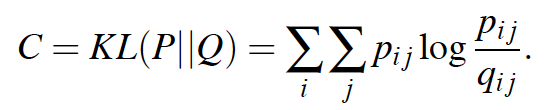
\includegraphics[scale=.3]{eq8}
	\caption{تابع هزینه متقاران}\label{fig.eq8}
\end{figure}
\\
که باز در این تابع نیز مقادیر $p_{ii}$ و $q_{ii}$ برابر با صفر هستند.
این نوع اس ان ای، اس ان ای متقارن شمرده می‌شود زیرا برای تمام $i$ و $j$ ها داریم که
$p_{ij} = p_{ji}$
و 
$q_{ij} = q_{ji}$
.
\\
در اس ان ای متقارن، شباهت بین دو نقطه نگاشت شده در ابعاد پایین با فرمول زیر محاسبه می‌شود:
 \begin{figure}[!h]
 	\centering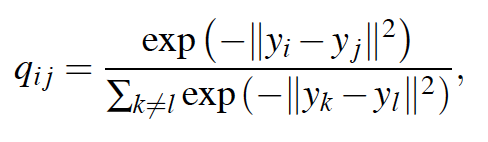
\includegraphics[scale=.3]{eq9}
 	\caption{تابع شباهت در ابعاد پایین}\label{fig.eq9}
 \end{figure}
\\
و همچنین تابع شباهت بین دو نقطه در ابعاد بالا نیز به فرمول زیر است:
\begin{figure}[!h]
	\centering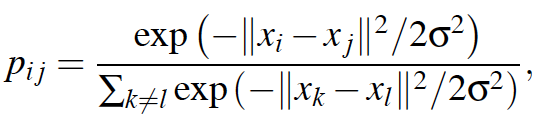
\includegraphics[scale=.3]{eq10}
	\caption{تابع شباهت در ابعاد بالا}\label{fig.eq10}
\end{figure}
\\
اما این فرمول در زمانی که یک داده در ابعاد بالا،
{داده‌ی پرت}\LTRfootnote{outlier}
باشد مشکل زا می‌شود زیرا مقدار $p_{ij}$ برای تمام $j$ های به غیر از این داده بسیار کم می‌شود و نگاشت آن به هر جایی از صفحه آنچنان تاثیری در تابع هزینه نخواهد داشت و در نتیجه مکان این نقطه نگاشت شده، به خوبی توسط بقیه نقاط مشخص نمی‌شود.
\\
برای دور زدن این مشکل، تابع شباهت در ابعاد بالا را به صورت میانگین دو تابع احتمال شرطی تعریف می‌کنیم، یعنی مقدار $p_{ij}$ را به صورت
$\frac{p_{j|i} + p_{i|j}}{2n}$
تعریف می‌کنیم. این تعریف تضمین می‌دهد که
$\sum_j {p_{ij}} > \frac{1}{2n}$
برای تمام
$x_i$
ها و در نتیجه هر نقطه، تاثیر بالایی در تابع هزینه $C$ خواهد داشت.
\\
تابع شباهت برای ابعاد پایین را تغییر نمی‌دهیم زیرا مشکل قبلی پیش نخواهد آمد.
\\
برتری اصلی اس ان ای متقارن نسبت به اس ان ای معمولی این است که تابع گرادیان آن بسیار ساده‌تر است که این موضوع باعث می‌شود که محاسبه‌ی آن بسیار سریع‌تر باشد. تابع گرادیان برای اس ان ای متقارن به شکل زیر است:
\begin{figure}[!h]
	\centering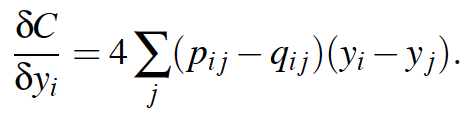
\includegraphics[scale=.3]{eq11}
	\caption{تابع گرادیان برای اس ان ای متقارن}\label{fig.eq11}
\end{figure}
\\
نتایج آزمایش‌ها نشان می‌دهد که اس ان ای متقارن قالبا همان نگاشت اس ان ای را خروجی می‌دهد و گاها عملکرد بهتری نیز ارائه می‌دهد.

\section{مشکل شلوغی}
مجموعه‌ای از نقاط دو بعدی را در نظر بگیرید، که بر روی یک منحی دو بعدی نامتقارن و دارای پستی و بلندی قرار دارند که در به صورت تقریبی می‌توان با یک خط در اندازه‌های کوچک تقریب زده شوند، و تمام این نقاط در فضایی با ابعاد بالا تعبیه شده‌اند.
این امکان وجود دارد که فاصله‌ی دو به دوی نقاط را در یک نگاشت دو بعدی مدل کرد.
\\
حال فرض کنید که پستی بلندی‌های واقعی منحنی که در نگاه جزئی دیده نمی‌شدند دارای ده بعد دیگر جز این دو بعد باشند که دیگر نمی‌توان آن‌ها را به خوبی در دو بعد مدل کرد. دلایل متنوعی برای این موضوع وجود دارد که برای مثال می‌توان گفت که در ۱۰ بعد، می‌توان ۱۱ نقطه را جوری در صفحه چید که فاصله‌ی بین آن‌ها را به هیچ صورتی نمی‌توان به خوبی در دو بعد نشان داد.
\\
یک مسئله مربوط به این موضوع، مسئله‌ی نگاشت یک ابر کره‌ی $m$ بعدی به دو بعد است که توزیع نقاط در آن به این صورت است که یک مرکز در نظر گرفته شده و احتمال وجود یه نقطه در مکانی که فاصله‌ی $r$ از مرکز دارد متناسب با $r^m$ می‌باشد، که برای حل این مسئله نیز به مشکل شلوغی می‌خوریم.
\\
مسئله شلوغی رو می‌توانیم به این صورت تعریف کنیم: فضای دو بعدی در دسترس برای نمایش فاصله‌ی نقاط نسبتا دور از هم به اندازه‌ی کافی بزرگتر از فضای دو بعدی در دسترس برای نمایش فاصله‌ی نقاط نزدیک به هم نیست، به همین دلیل ما اگر بخواهیم فاصله‌ی نقاط نزدیک به هم را به خوبی نگاشت دهیم، نقاط نسبتا دور از هم در نگاشت، بسیار دور از هم نگاشت داده می‌شوند.
\\
در اس ان ای، فنری که بین این داده‌ی $i$ و هر یک از این داده‌های بسیار دور نگاشت داده شده، قرار داده شده است، بسیار  سختی پایینی دارد و به همین دلیل نیروی جذبی ضعیفی از خود نشان می‌دهد.
\\
اگرچه این فنرها نیروهای بسیار ضعیفی از خود نشان می‌دهند اما تعداد زیادی از این نیرو‌ها داده‌ها را به سمت مرکز حرکت می‌دهد که باعث می‌شود فاصله‌ی طبیعی بین خوشه‌ها از بین برود.
\\
دقت کنید که این مشکل فقط مربوط به اس ان ای نمی‌باشد و در روش‌های دیگر نیز پیش می‌آید.
\\
یک تلاش برای حل مشکل شلوغی، اضافه کردن یک دافعه خفیف به هر فنر می‌باشد.
\\
این دافعه خفیف به این شکل ساخته می‌شود که یک مدل پس‌زمینه یکنواخت با نسبت اختلاط $\rho$ معرفی می‌شود. که در آن نقاط نگاشت داده شده‌ی بسیار دور از هم مقدار $q_{ij}$ کمتر از 
$\frac{2p}{n(n-1)}$
نمی‌توانند داشته باشند که در نتیجه‌ی آن نقاطی که در ابعاد بالا بسیار دور هستند مقدار $q_{ij}$ آن‌ها همواره بیشتر از مقدار $p_{ij}$ آن‌ها می‌شود که این موضوع باعث یک دافعه خفیف می‌شود.
\\
به این روش
{یونی اس ان ای}\LTRfootnote{UNI-SNE}
می‌گویند که گرچه بسیار بهتر از روش اس ان ای عمل می‌کند اما تابع هزینه‌ی آن بسیار پیچیده است.
\section{دم نامناسب می‌تواند ابعاد ازبین رفته را جبران کند}
از آنجایی که روش اس‌ان‌ای متقارن تلاش می‌کند تا توزیع توأم در ابعاد بالا و پایین را برابر یک‌دیگر قرار دهد، راه حل مناسبی برای حل مشکل گزارش شده در زیر بخش قبل وجود دارد که به شرح زیر است.
در ابعاد بالا برای تبدیل فاصله به احتمال از توزیع گوسی استفاده‌شده‌است اما در ابعاد‌پایین می‌توان از توزیع احتمالی استفاده کرد که فاصله خطی بیش‌تری را نسبت به توزیع گوسی ایجاد کند. با این‌روش فاصه‌های که متوسط هستند نیز در ابعاد کوچک به فاصله‌های بزرگ‌تر مپ می‌شوند و به طبع باعث می‌شود که آن‌های که در یک خوشه نیستند شباهت احتمالی کمتری داشته‌باشند و نمایش بهتری داشته باشیم.

\section{روش‌های بهینه‌سازی برای تی-اس‌ان‌ای}
در ابتدا روش تی-‌اس‌ان‌ای با استفاده از الگوریتم گرادیان‌دسنت روی تابع‌هزینه بهینه‌سازی شد. شبه کد نحوه‌ی بهینه سازی آن در\cref{algfig1} آورده شده است.
\\
\begin{figure}
	\centering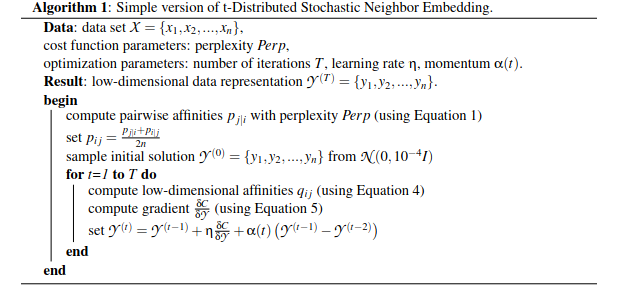
\includegraphics[scale=.6]{algfig1.png}
	\caption{شبه کد بهینه سازی }\label{algfig1}
\end{figure}

این الگوریتم ساده این قابلیت‌را دارد تا با استفاده از  نرخ‌یادگیری‌انطباقی که در سال ۱۹۸۸ توسط جکابس \LTRfootnote{Jcobs }معرفی شد، که در آن نرخ یادگیری را درجهتی که گرادیان ثابت بماند، نرخ یادگیری را زیاد‌میکرد ،سریع‌تر شود.
\\
هرچند این الگوریتم تصاویری ایجاد می‌کند که بسیار بهتر از دیگر الگوریتم‌های غیر‌پارامتریک هستند،  می‌توان از طریق دو ایده‌ای که در این بخش معرفی‌می‌کنیم تصاویر بسیار بهتری ایجاد کرد.
اولین ایده که آن‌را فشرده‌سازی‌اولیه \LTRfootnote{early compression} می‌نامیم تلاش می‌کند تا در همان‌ابتدای بهینه‌سازی نقاط را نزدیک به‌هم نگه‌دارد. با این روش فاصله نقاط به یکدیگر کوچک می‌شوند و به این‌ترتیب نقاط داخل یک خوشه راحت همدیگر‌را پیمایش می‌کنند. برای انجام فشرده‌سازی‌اولیه یک پارامتر به‌نام $L2-penalty$ را به تابع هزینه اضافه می‌کنیم. که متناسب است با مجذور مجوع جمع فاصله‌نقاط در فاصله اصلی. 
\\
روش دوم به‌نام  مبالغه‌اولیه \LTRfootnote{early exaggeration} که کمی پیچیده‌تر از روش اول است به این ترتیب می‌باشد که در آن همه پارامتر‌های
$P_{ij}$
را در یک عددی مانند ۴ در‌همان گام‌های نخست ضرب می‌کنیم.
. با انجام این‌کار 
$q_{ij}$
ها که هنوز جمع آن‌ها برابر یک است بسیار کوچک تر از 
$P_{ij}$
ها می‌باشند و این باعث می‌شود که مدل تلاش کند اعداد بسیار بزرگ
$p_{ij}$
را به اعداد بزرگ‌ترین اعداد 
$q_{ij}$
نگاشت کند و به‌تبع باعث خوشه‌بندی بهتری برای در‌ابعاد پایین می‌شود.
\\
در تمامی آزمایش‌های انجام شده در این مقاله از بهینه‌سازی ذکر‌شده همراه با مبالغه‌اولیه با عدد ۴ برای ۵۰ تکرار اول بهینه‌سازی استفاده شده است.نرخ یادگیری نیز همانطور که ذکر شد به روش انطباقی در طول تکرار تغییر کرد.

% \chapter{آزمایش‌ها}
برای بررسی عملکرد الگوریتم تی-اس-ای \LTRfootnote{t-SNE}  با دیگر الگوریتم‌های زیر مورد مقایسه قرار داده شده است.
\begin{itemize}
	\item $Sammon mapping$
	\item $Isomap$
	\item $LLE$
	\item $CCA$
	\item $SNE$
	\item $MVU$
	\item $ Laplacian Eigenmaps.$
\end{itemize}
این مقایسه برای پنج دیتاست انجام شده که در مقاله به سه مجموعه داده اشاره می‌شود که در زیر آورده شده است.
\section{دیتاست‌ها}
پنج دیتاستی که مقایسه روی آن‌ها انجام شده است عبارتند از :
\begin{itemize}
	\item دیتاست $MNIST$
	\item دیتاست $Olivetti faces$
	\item دیتاست $COIL\-20$
	\item دیتاست مربوط به کلمات.
	\item دیتاست نتفلیکس.
\end{itemize}.
\\
در این بخش سه دیتاست اول را مورد بررسی قرار میدهیم. 
\\
دیتاست اول دارای شصت‌هزار عکس از اعداد دست‌نوشته می‌باشد. برای این‌ آزمایش شش ‌هزار تصویر به صورت تصادفی برای بار محاسبتی کمتر انتخاب شده اند. هر تصویر شامل ۷۶۸ پیکسل می‌باشد.دیتاست دوم شامل ۴۰۰ تصویر از ۴۰ لیوان مختلف از هر لیوان ۱۰ تصویر و هر تصویر دارای ۱۰۳۰۴ پیکسل می‌باشد که هر تصویر با توجه به مشخصاتی که دارا بود برچسب خورده است. دیتاست سوم نیز شامل ۱۴۴۰ تصویر با ابعاد ۳۲ در ۳۲ می‌باشد که از ۲۰ شی مختلف تصویر برداری شده است.

\section{نحوه‌آزمایش}
در این آزمایش در ابتدا همه دیتاست‌ها با استفاده از $pca$ به ۳۰ بعد کاهش یافته اند. این کار به دلیل بار محساباتی کمتر صورت گرفته است. همچنین همه نقاط در سه دیتاست رنگ‌بندی شده اند. این رنگ بندی صرف فهمیدن بهتر نحوه عملکرد الگوریتم‌ها صورت گرفته است.
\\
پارامتر‌های تابع هزینه هر الگوریتم در زیر معرفی شده است.
\begin{itemize}
	\item الگوریتم $t\-SNE$: در این الگوریتم پارامتر سرگشتی توزیع شرطی احتمال که توسط کرنل گوسی استفاده شده برابر 40 قرار داده شده است.
	\item الگوریتم $sammon mapping$: در این الگوریتم متد نیوتون با ۵۰۰ بار تکرار انجام شده است..
	\item الگوریتم $Isomap$ و $LLE$ : در این دو الگوریتم عدد $k$  مربوط به تعداد همسایگان نزدیک در گراف همسایگی ۱۲ در نظر گرفته شده است.
\end{itemize}.
\\
\section*{نتایج}
در زیر تصاویر مربوط به نتایج آورده شده است .تصاویر به وضوح عملکرد مناسب$t\-SNE$ را نشان‌میدهد در به‌صورتی که تصویر مربوط به دیتاست اول دو الگوریتم $ISomap$ و $LLE$ باعث شده‌اند داده‌ها در بعد پایین هم‌پوشانی بالایی داشته‌باشند اما در الگوریتم $sammon mapping$ تنها سه کلاس از داده های کلاستر شده از‌هم جدا باشند و دیگر داده‌ها مشابه شوند ولی در مقابل الگوریتم معرفی شده توانسته است تا حد قابل قبولی داده‌های مشابه را نسب به دیگر داده‌ها نزدیک تر قرار دهد.

\begin{figure}
	\centering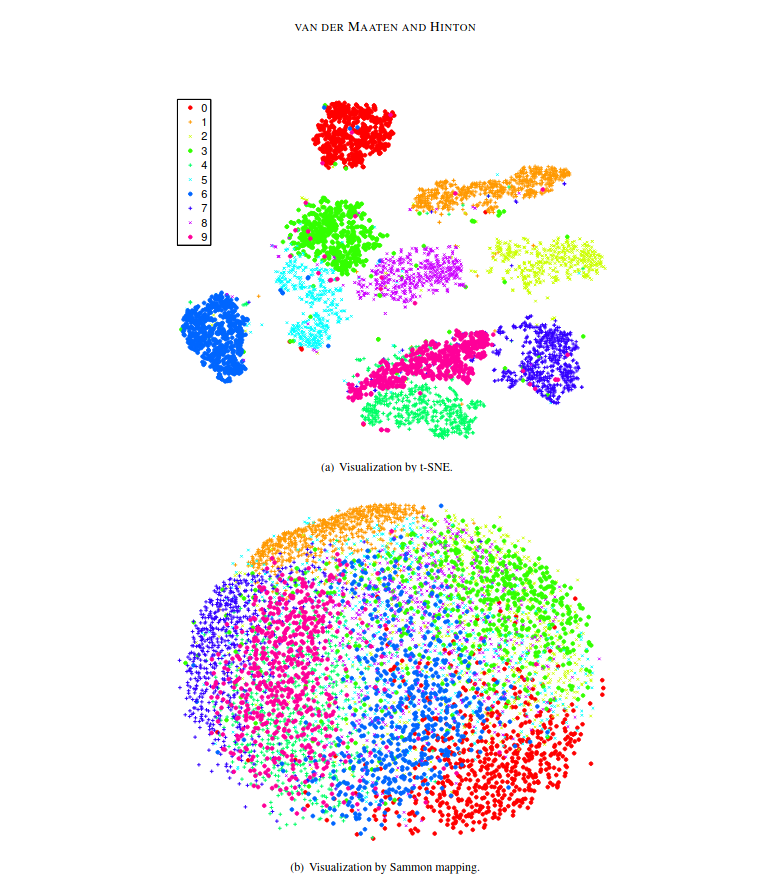
\includegraphics[scale=.6]{resfig1.png}
	\caption{نمایش ۶۰۰۰ هزار تصویر اعداد ۱ تا ۹ به صورت دست‌نویس از دیتاست اول}\label{resfig.1}
\end{figure}

\begin{figure}
	\centering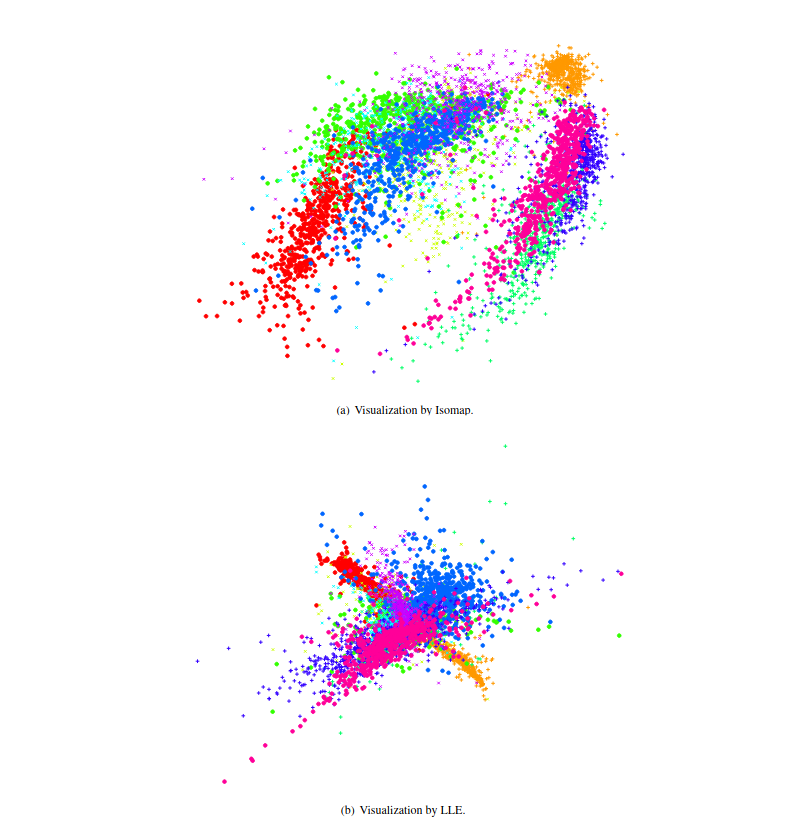
\includegraphics[scale=.6]{resfig2.png}
	\caption{نمایش ۶۰۰۰ هزار تصویر اعداد ۱ تا ۹ به صورت دست‌نویس از دیتاست اول}\label{resfig.2}
\end{figure}

\begin{figure}
	\centering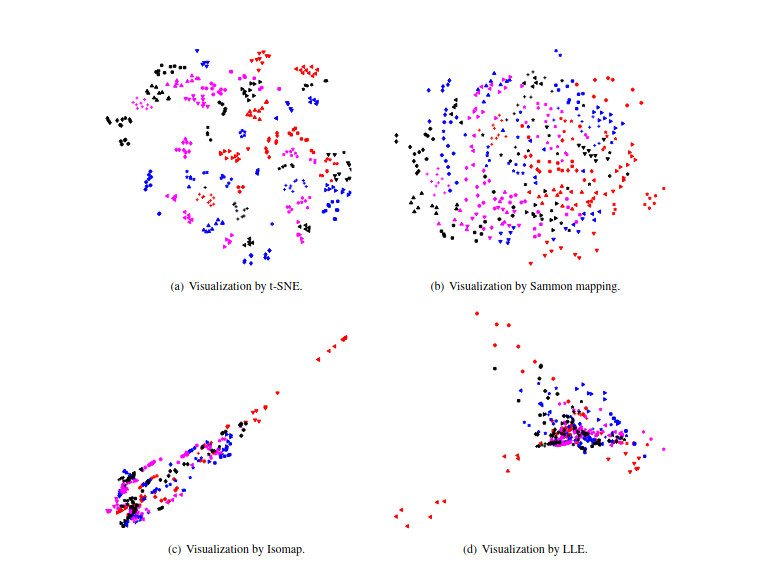
\includegraphics[scale=.6]{resfig3.png}
	\caption{مقایسه الگوریتم‌ها در دیتاست دوم}\label{resfig.3}
\end{figure}

\begin{figure}
	\centering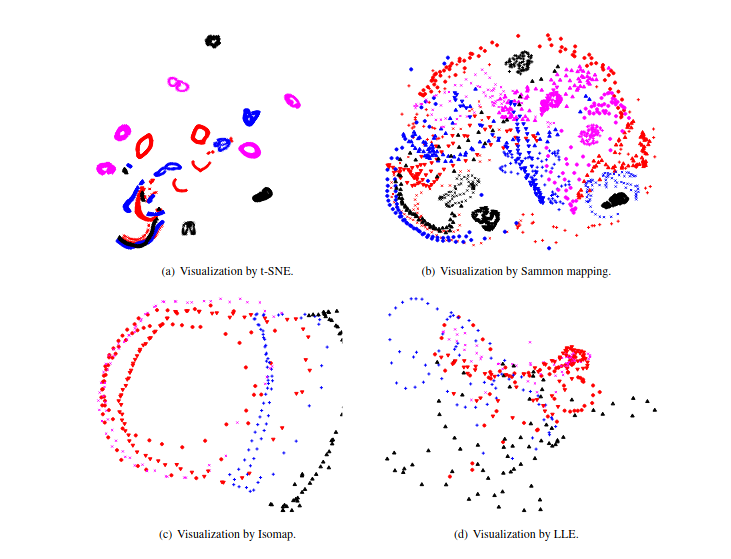
\includegraphics[scale=.6]{resfig4.png}
	\caption{مقایسه الگوریتم‌ها در دیتاست سوم}\label{resfig.4}
\end{figure}
سه مقایسه بالا نشان داد دیگر الگوریتم‌ها به خوبی $t\-SNE$ معرفی شده کار نمی‌کنند همچنین لازم به ذکر است که با توجه به محاسبات الگوریتم‌های $Isomap$ و  $LLE$  در دیتاست دوم ، اعداد حاصل در نزدیک بودن کلاس‌های معرفی شده بسیار بزرگ بوده و باعث شده‌است که حتی نتواند انها در  داخل یک دسته نگه دارد.


% \chapter{ به‌کارگیری تی‌اس‌ان‌ای بر روی مجموعه داده‌های بزرگ}
%%%%%%%%%%%%%%%%%%%%%%%%%%%%%%%%%%%%%%%%%%%
\section*{جمع‌بارگیری تی‌اس‌ان‌ای بر روی مجموعه داده‌های بزرگ}
مانند بسیاری دیگر از تکنیک‌های مصورسازی داده، تی‌اس‌ان‌ای از نظر پیچیدگی زمان و حافظه به نسبت تعداد داده‌های درجه 2 است. این امر باعث می‌شود تا اعمال این الگوریتم بر روی‌مجموعه داده‌هایی که بیش از ۱۰۰۰۰ دارند غیر ممکن شود. مشخصا نمونه برداری از روی داده‌ها یک راه حل ممکن برای رفع این مشکل است؛ اما این روش نمی‌تواند از اطلاعاتی که داده‌های انتخاب نشده در نمونه برداری در مورد گوناگونی داده‌های دیتاست در اختیار ما می‌گذارند بهره ببرد. به عنوان مثال فرض کنید داده‌های
 $A$، $B$، $C$
  در فضای چند بعدی به صورت دو به دو فاصله‌ی یکسانی از یکدیگر داشته باشند. اگر تعداد زیادی داده‌ی نمایش داده نشده در بین $A$ و $C$ وجود داشته باشد اما تمام داده‌های بین $A$ و $B$ در نمونه برداری موجود باشند، آنگاه احتمال اینکه $A$ و $B$ بخشی از یک خوشه باشند بسیار بیش‌تر از احتمال هم خوشه بودن $A$ و $C$ است. این امر در \cref{chapfig3} نشان داده شده است. در این بخش نشان خواهیم داد که تی‌اس‌ان‌ای چگونه می تواند تغییر کند تا با نشان دادن یک زیرمجموعه تصادفی از داده‌ها بتواند از تمام اطلاعات مربوط به تنوع داده‌های دیتاست اصلی استفاده نماید.
\\

\begin{figure}
	\centering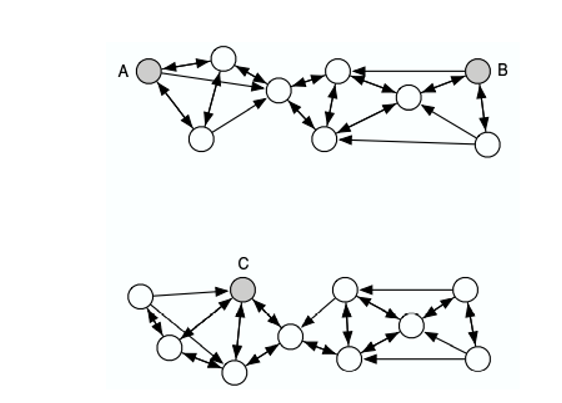
\includegraphics[scale=.6]{chapfig3.PNG}
	\caption{ }\label{chapfig3}
\end{figure}
\begin{figure}
	\centering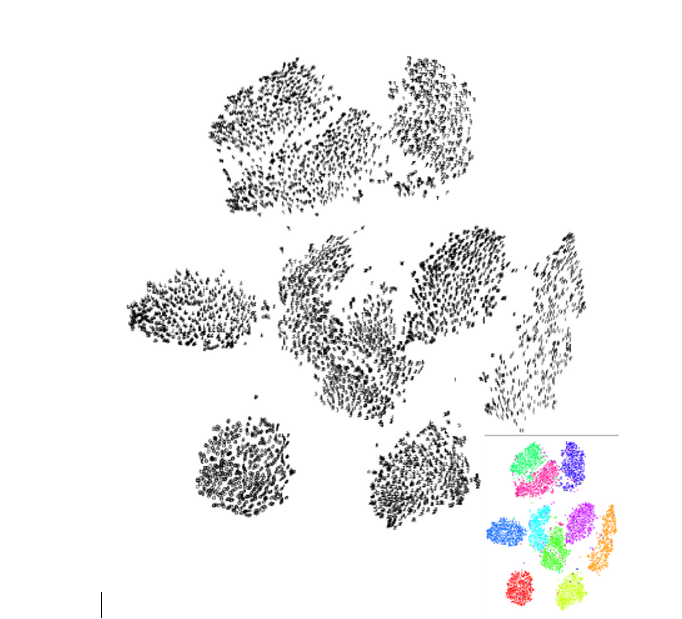
\includegraphics[scale=.6]{chapfig2.PNG}
	\caption{ }\label{chapfig2}
\end{figure}


به کارگیری تی‌اس‌ان‌ای بر روی مجموعه داده‌های بزرگ
برای این‌ کار، ابتدا یک تعداد مشخص از نقاط همسایه را در نظر می‌گیریم و یک گراف همسایگی برای تمام داده‌ها می‌سازیم. اگرچه این کار بار محاسباتی بسیار زیادی دارد، اما قرار است تنها یک بار این فرایند را انجام دهیم. سپس از هر نقطه برجسته ، به طور تصادفی شروع به قدم زدن بر روی گراف همسایگی می‌کنیم تا به یک نقطه برجسته دیگر برسیم. در حین قدم زدن تصادفی، احتمال انتخاب هر یال که از نقطه
 $x_i$
  شروع و به نقطه $xj$ ختم می‌شود، متناسب است با
$e^{‖x_i-x_j ‖^2}$
. مقدار
$ P_{j|i}$
 برابر است با بزرگی نسبی تعداد قدم‌های تصادفی که از نقطه‌ی برجسته‌ی$ x_i$ شروع شده وبه نقطه‌ی برجسته‌ی$ x_j$ ختم می‌شود. این تعریف شباهت‌هایی با روش $Isomap$ دارد که شباهت دو به دوی نقاط را اندازه‌گیری می‌کند. با این حال، همانند نقشه‌های انتشار، به جای اینکه به دنبال کوتاه ترین مسیر در گراف همسایگی باشیم، مقیاس نزدیکی بر مبنای قدم زدن تصادفی برای تمام مسیرها با یکدیگر ادغام می‌شوند. بنابراین، مقیاس نزدیکی بر مبنای قدم زدن تصادفی، در برابر مسیرهای کوتاهی که توسط داده‌های نویز ساخته شده‌اند یعنی $"short circuiting"$مقاوم است. (تعدادی داده‌ی نویز می‌توانند یک مسیر کوتاه بین دو خوشه جدا از هم بسازند که باعث متصل شدن دو خوشه می‌شود.)


بدیهی ترین روش برای محاسبه میزان شباهت بر مبنای قدم زدن تصادفی این است که به طور مستقیم قدم زدن تصادفی را بر روی گراف همسایگی اجرا کنیم که این روش در عمل بسیار کابردی است، چراکه می‌توان در هر ثانیه حدود یک میلیون بار قدم زدن را اجرا کرد. در روشی دیگر، یک راه حل تحلیلی برای محاسبه‌ی دو به دوی شباهت‌ها ارائه می‌شود که شامل حل کردن یک مدل خطی غیر متراکم است.  در تجربه‌های اولیه، چندان تفاوتی میان اجرای مستقیم قدم زدن تصادفی و روش‌های تحلیلی مشاهده نمی‌‌شود. در آزمایشی که در این بخش به آن می‌پردازیم، برای محاسبه شباهت‌ها به اجرای مستقیم قدم زدن تصادفی روی می‌آوریم چراکه بار محاسباتی کمتری دارد. اما در نظر داشته باشید که برای دیتاست‌های بسیار بزرگ که ممکن است نقاط استراژیک بسیار پراکنده باشند، روش‌های تحلیلی کارآمد تر خواهند بود. \cref{chapfig2} نتیجه یک آزمایش را نشان می‌دهد که در آن برای محاسبه دو به دوی شباهت‌ها، قدم زدن تصادفی را بر روی یک مجموعه‌ی شش هزارتایی از داده‌ها که به طور تصادفی از میان یک دیتاست شصت هزارتایی انتخاب شده‌اند اجرا شده است. در این آزمایش، از یک گراف همسایگی استفاده شده است که به ازای مقدار $K=20$ ساخته می‌شود؛ یعنی بیست تا از نزدیکترین همسایه‌های هر نقطه انتخاب می‌شوند. قسمت داخلی شکل، کل دیتاست را نشان می‌دهد که هر کلاس با یک رنگ خاص و متفاوت نشان داده شده است. در نقشه تی‌اس‌ان‌ای کاملا می‌توان مشاهده کرد که کلاس‌های مختلف به خوبی از یکدیگر قابل تفکیک می‌باشند و علاوه بر آن، واریانس و شکل خوشه‌ها به خوبی حفظ شده است. عملکرد بسیار خوب   تی‌اس‌ان‌ای را می‌توان از خطای تعمیم  \LTRfootnote{generalization error} محاسبه شده برای الگوریتم $KNN$ نیز مشاهده کرد. در حالیکه خطای تعمیم برای الگوریتم $KNN$ به ازای $K=1$ که بر روی دیتاست اصلی آموزش دیده است برابر 5.75 درصد است، مقدار این خطا برای همین الگوریتم که بر روی دیتاست‌ای که توسط تی‌اس‌ان‌ای تولید شده است آموزش دیده، برابر 5.13 درصد است. بار محاسباتی برای اجرای قدم زدن تصادفی تی‌اس‌ان‌ای بسیار معقول است. به طوریکه تنها یک ساعت زمان برای تولید \cref{chapfig2} لازم است.


% \chapter{بررسی نهایی}
نتیجه‌های بدست آمده در دو بخش قبلی، کارایی تی‌اس‌ان‌ای را بر روی چندین مجموعه مختلف از دیتاست‌ها به خوبی نشان داد. در این بخش قصد داریم تا تی‌اس‌ان‌ای را با چندین تکنیک مطرح دیگر مقایسه کنیم و تفاوت‌های آن را بیان نماییم. همچنین به برخی از نقاط ضعف تی‌اس‌ان‌ای اشاره کرده و مواردی را برای ارتقای این روش ارائه می-کنیم.

\section{مقایسه با دیگر تکنینک‌ها}

امروزه پیروش
مقیاس بندی کلاسیک\LTRfootnote{ classical scaling }
که بسیار نزدیک به ‌$pca$ است، به دنبال یک انتقال خطی می‌گردد که مجموع مربعات خطاها\LTRfootnote{SSE} را مینیمم کند. خطاها به صورت فاصله‌ی دو به دوی داده‌ها در فضای بالاتر و تبدیلشان در فضای پایین تر تعریف می‌شوند. یک مدل خطی مانند مقیاس بندی کلاسیک، نمی‌تواند خوشه‌های منحنی مانند را به خوبی مدل کند، چراکه تمرکز آن بیش‌تر بر روی حفظ فاصله‌ی داده‌های جدا از هم است و توجهی به حفظ فاصله‌ی داده‌ی نزدیک به هم ندارد. یک روش مهم که سعی در بر طرف کردن مشکلات مقیاس بندی کلاسیک دارد، روش نقشه برداری 
سامون\LTRfootnote{sammon} 
می‌باشد که تابع هزینه را به صورت تقسیم فاصله‌ی اقلیدسی دو به دوی داده‌های انتقال داده شده به فاصله‌ی اقلیدسی آن‌ها در فضای اصلی تعریف می‌کند. بنابراین تابع هزینه برابر خواهد بود با فرمول \cref{chapfig4}
\begin{figure}
	\centering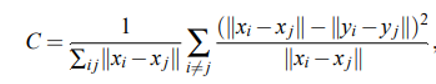
\includegraphics[scale=.6]{chapfig4.PNG}
	\caption{ }\label{chapfig4}
\end{figure}

که کسر بیرون از علامت سیگما برای ساده سازی گرادیان تابع نوشته شده است. نقطه ضعف اصلی این تابع هزینه این است که حفظ داده‌های با فاصله نزدیک تا حد زیادی به اندازه فاصله دو به دوی آن‌ها وابسته است. به نحوی که اگر یک خطای کوچک در مدل سازی دو داده‌ای که بسیار به یکدیگر نزدیک هستند رخ دهد، منجر به افزایش تابع هزینه به مقدار زیادی خواهد شد. از آنجایی که تمام فواصل دو به دو در شکل دهی فرم‌های محلی نقش دارند، بهتر است تا اهمیتی تقریبا برابر به فواصل به اندازه کافی کوچک داده شود. 
\\
در مقابل روش $Sammon$، روش کرنل گوسی  \LTRfootnote{ Gaussian kernel } وجود دارد که توسط تی‌اس‌ان‌ای در ابعاد بالا به کار گرفته می‌شود. این روش یک حاشیه نرم بین فرم‌های محلی ایجاد می‌کند و برای جفت‌هایی که بر مبنای انحراف معیار مدل گوسی به یکدیگر نزدیک می‌باشند، اهمیت بیش‌تری در نظر گرفته می‌‌شود. بنابراین اهمیت حفظ هر فاصله، مستقل از بزرگی آن است. علاوه بر آن، تی‌اس‌ان‌ای تعداد همسایگان محلی را برای هر داده به طور جداگانه و بر مبنای چگالی محلی مشخص می-کند.
برتری کارایی تی‌اس‌ان‌ای در مقایسه با $Isomap$ در بحث مقاوم بودن در برابر             $"short circuiting"$ به خوبی نشان داده شد. علاوه بر آن، $Isomap$ بر روی حفظ ساختارهای بزرگ داده تمرکز دارد در حالی که تی‌اس‌ان‌ای به حفظ فرم‌های محلی بیش‌تر اهمیت می‌دهد.
عملکر قوی تی‌اس‌ان‌ای در مقایسه با $LLE$، به یک نقطه ضعف بزرگ در $LLE$ باز می‌گردد: تنها عاملی که باعث می‌شود تا تمام داده‌ها در یک خوشه قرار نگیرند محدودیتی است که بر روی کوواریانس داده‌ها انتقال داده شده اعمال می‌شود. در عمل این محدودیت می‌تواند با قرار دادن تمام داده‌ها حول یک مرکز و چندین داده‌ی متراکم که فاصله‌ی آن‌ها از مرکز به نسبت بقیه داده‌ها بسیار زیاد است به سادگی ارضا شود. محدودیت کوواریانس در گراف همسایگی نیز می‌تواند با وجود چند ناحیه متراکم و جدا از هم ارضا شود. بنابراین روش $LLE$ نمی‌تواند ناحیه‌های متراکم که شامل چند خوشه هستند ولی از یکدیگر دور اند را به خوبی مدل کند. به عنوان مثال  \cref{chapfig1} را در نظر بگیرید، $LLE$ قادر به تفکیک خوشه‌های قرمز و آبی و همچنین خوشه‌های زرد و سبز نخواهد بود و کل دیتاست را به دو خوشه دسته بندی می‌کند. 
همانند $LLE$ ، قدم زدن تصادفی در تی‌اس‌ان‌ای از گراف همسایگی استفاده می‌کند اما مشکلات $LLE$ را نخواهد داشت چراکه شباهت دو به دوی داده‌ها در فضای اصلی، با در نظر گرفتن ترکیبی از تمام مسیرهای بین دو داده در گراف همسایگی مشخص می-شود.


\begin{figure}
	\centering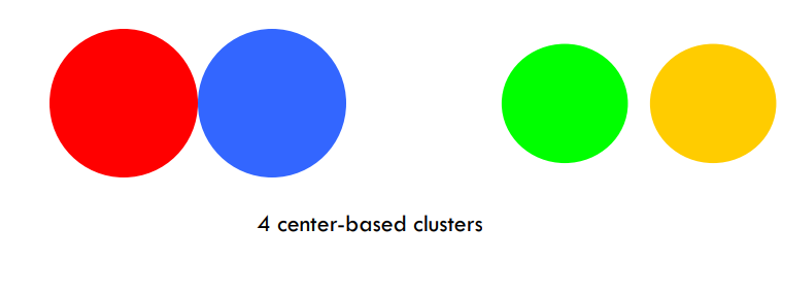
\includegraphics[scale=.6]{chapfig1.PNG}
	\caption{ }\label{chapfig1}
\end{figure}

\section{نقاط ضعف}
اگرچه در قسمت قبل مشاهده کردیم که تی‌اس‌ان‌ای نسبت به برخی روش‌های دیگر برتری هایی دارد اما این روش دارای نقطه ضعف‌هایی نیز می‌باشد که اصلی ترین آن‌ها عبارت‌اند از: (‌۱) مشخص نیست که تی‌اس‌ان‌ای در کاهش ابعاد دقیقا چگونه عمل می-کند. (۲) کاهش ابعاد بر مبنای ویژگی‌های محلی داده‌ها، باعث می‌شود تا تی‌اس‌ان‌ای نبت به ابعاد ذاتی داده‌ها حساس باشد. (۳) تابع هزینه تی‌اس‌ان‌ای محدب نیست و بنابراین تضمینی وجود ندارد که به بهینه ترین حالت برسیم. در ادامه به طور خلاصه به شرح این نقاط ضعف می‌پردازیم.
\begin{itemize}
\item 	کاهش ابعاد برای اهداف دیگر: مشخص نیست که روش تی‌اس‌ان‌ای  در حالت کلی دقیقا چگونه ابعاد را کاهش می‌دهد. این روش برای کاهش ابعاد داده‌ها به دو یا سه بعد مناسب است اما در حالتی که نیاز داشته باشیم ابعاد داده‌ها بیش‌تر از سه بعد باشد، بهتر است از آن استفاده نکنیم چراکه نمی‌تواند به خوبی داده‌‌ها را مدل کند. بنابراین اگر شرایط به گونه ای باشد که برای حفظ فرم و اطلاعات کلی داده‌ها به بیش‌تر از سه بعد نیاز باشد، تی‌اس‌ان‌ای کارایی لازم را نخواهد داشت.
\item 	نفرین ابعاد ذاتی: تی‌اس‌ان‌ای ابعاد داده‌ها بر مبنای ویژگی‌های محلی دیتاست کاهش می‌دهد که این امر می‌تواند آن را در مقابل دیتاست‌هایی که ابعاد ذاتیشان بالا است و تنوع نواحی مختلف آن‌ها زیاد است، آسیب پذیر کند. روش‌های $LLE$ و $Isomap$ هم دارای همین مشکل هستند.
\item	غیر محدب بودن تابع هزینه تی‌اس‌ان‌ای: تابع هزینه در تی‌اس‌ان‌ای محدب نمی‌باشد بنابراین تضمینی وجود ندارد که به بهینه ترین حالت ممکن برسیم چراکه باید پارامترهای بهینه سازی زیادی را بیابیم که در هر اجرا و آزمایش متفاوت خواهند بود. اما این نقطه ضعف نمی‌تواند دلیلی برای کنار گذاشتن تی‌اس‌ان‌ای و استفاده از روش‌های $LLE$ و $Isomap$ که تابع هزینه آن‌ها محدب است باشد. چراکه رسیدن به مینیمم نسبی یک تابع هزینه که ویژگی‌های داده‌ها را به وطور قابل قبولی منعکس می‌کند، بهتر از رسیدن به مینیمم مطلق تابعی است که نمی‌تواند اطلاعات مد نظر دیتاست را مدل کند. به علاوه، محدب بودن تابع هزینه به این معنا نیست که حتما می‌توان به بهینه ترین حالت ممکن رسید. چراکه محاسبه مینیمم مطلق توابع هزینه در بسیاری از تجربه‌های واقعی از نظر بار محاسباتی غیر ممکن است.
\end{itemize}

\section{نتیجه گیری}
در این مقاله، یک تکنیک جدید برای مصور سازی داده‌ها معرفی شد که می‌تواند ویژگی-های محلی داده‌های نزدیک به هم را به خوبی منعکس کند و علاوه بر آن بخشی از اصلی ترین ویژگی‌های سراسری دیتاست را نیز حفظ نماید. پیچیدگی حافظه و زمان روش تی‌اس‌ان‌ای برابر $O(n^2)$ است. اما رویکرد شاخصی در این مقاله مطرح شد که اجرای تی‌اس‌ان‌ای را بر روی دیتاست‌های بزرگ ممکن می‌کند. تجربه‌های بدست آمده از اجرای تی‌اس‌ان‌ای بر روی چندین دیتاست مختلف نشان داد که این روش به نسبت برخی روش‌های مطرح دیگر در زمینه مصور سازی داده بهتر عمل می‌کند.
برای ارتقای این روش در آینده قصد داریم تا بهینه سازی را بر روی تعداد درجات آزادی توزیع $t\-Student$ (که در تی‌اس‌ان‌ای استفاده می‌شود) پیاده سازی کنیم. این کار به برطرف کردن اولین نقطه ضعف مطرح شده در قسمت قبل کمک می‌کند. همچنین گسترش تی‌اس‌ان‌ای را به گونه‌ای که هر داده در فضای بالاتر بتواند به چندین داده در فضا پایین‌تر مدل شود، بررسی خواهیم کرد.  به علاوه، هدف ما توسعه‌ی یک نسخه پرامتری از تی‌اس‌ان‌ای است که در آن با استفاده از تابع هدف تی‌اس‌ان‌ای ، به آموزش یک شبکه عصبی چند لایه‌ای که یک نگاشت مستقیم از فضای اصلی به یک فضای با ابعاد کمتر را فراهم می‌کند، می‌پردازیم. 



%--------------------------------------------------------------------------appendix( مراجع و پیوست ها)
\chapterfont{\vspace*{-2em}\centering\LARGE}%

\appendix
% \bibliographystyle{plain-fa}
% \bibliography{references}
%\chapter*{‌پیوست}
\markboth{پیوست}{}
\addcontentsline{toc}{chapter}{پیوست}
موضوعات مرتبط با متن گزارش پایان نامه كه در يكی از گروه‌های زير قرار می‌گيرد، در بخش پيوست‌ها آورده شوند:
\begin{enumerate}
\item  اثبات های رياضی يا عمليات رياضی طولانی‌.‌
\item داده و اطلاعات نمونه (های) مورد مطالعه (\lr{Case Study}) چنانچه طولانی باشد‌.‌
\item نتايج كارهای ديگران چنانچه نياز به تفصيل باشد‌.‌
\item مجموعه تعاريف متغيرها و پارامترها، چنانچه طولانی بوده و در متن به انجام نرسيده باشد‌.‌
\end{enumerate}
% براي شماره‌گذاري روابط، جداول و اشكال موجود در پيوست‌ از ساختار متفاوتي نسبت به متن اصلي استفاده مي‌شود كه در زير به‌عنوان نمونه نمايش داده شده‌است. 
% \begin{equation}
%F=ma
%\end{equation}
\section*{کد میپل }
\begin{latin}
\begin{verbatim}

with(DifferentialGeometry):
with(Tensor):
DGsetup([x, y, z], M)
																	frame name: M
a := evalDG(D_x)
																	D_x
b := evalDG(-2 y z D_x+2 x D_y/z^3-D_z/z^2)


\end{verbatim}
\end{latin}
%--------------------------------------------------------------------------dictionary(واژه نامه ها)
%اگر مایل به داشتن صفحه واژه‌نامه نیستید، خط زیر را غیر فعال کنید.
%\parindent=0pt
%%
\chapter*{واژه‌نامه‌ی فارسی به انگلیسی}
\pagestyle{style9}

\addcontentsline{toc}{chapter}{واژه‌نامه‌ی فارسی به انگلیسی}
%%%%%%
\begin{multicols*}{2}

{\bf آ}
\vspace*{3mm}


\farsiTOenglish{اسکالر}{Scalar}


\vspace*{3mm}
{\bf ب}
\vspace*{3mm}

\farsiTOenglish{بالابر}{Lift}


\vspace*{3mm}
{\bf پ}
%%\vspace*{3mm}

\farsiTOenglish{پایا}{Invariant}



\vspace*{3mm}
{\bf ت}
%%\vspace*{3mm}

\farsiTOenglish{ تناظر }{Correspondence}


\vspace*{3mm}
{\bf ث}
%%\vspace*{3mm}

\farsiTOenglish{ثابت‌ساز}{Stabilizer}

\vspace*{3mm}
{\bf ج}
%%\vspace*{3mm}

\farsiTOenglish{جایگشت}{Permutation}



\vspace*{3mm}
{\bf چ}
%%\vspace*{3mm}


\farsiTOenglish{چند جمله‌ای }{Polynomial}

\vspace*{3mm}
{\bf ح}
%%\vspace*{3mm}

\farsiTOenglish{حاصل‌ضرب دکارتی}{Cartesian product}


\vspace*{3mm}
{\bf خ}
%%\vspace*{3mm}

\farsiTOenglish{خودریختی}{Automorphism}

\vspace*{3mm}
{\bf د}
%%\vspace*{3mm}

\farsiTOenglish{درجه}{Degree}


\vspace*{3mm}
{\bf ر}
%%\vspace*{3mm}


\farsiTOenglish{ریزپردازنده}{microprocessor}


\vspace*{3mm}
{\bf ز}
%%\vspace*{3mm}


\farsiTOenglish{زیرمدول}{Submodule}


\vspace*{3mm}
{\bf س}
%%\vspace*{3mm}

\farsiTOenglish{سرشت}{Character}


\vspace*{3mm}
{\bf ص}
%%\vspace*{3mm}

\farsiTOenglish{صادقانه}{Faithful}

\vspace*{3mm}
{\bf ض}
%%\vspace*{3mm}

\farsiTOenglish{ضرب داخلی}{Inner product}

\vspace*{3mm}
{\bf ط}
%%\vspace*{3mm}


\farsiTOenglish{طوقه}{Loop}


\vspace*{3mm}
{\bf ظ}
%%\vspace*{3mm}


\farsiTOenglish{ظرفیت}{Valency}
 
\vspace*{3mm}
{\bf ع}
%%\vspace*{3mm}


\farsiTOenglish{عدم مجاورت}{Nonadjacency}



\vspace*{3mm}
{\bf ف}
%%\vspace*{3mm}

\farsiTOenglish{فضای برداری}{Vector space}



\vspace*{3mm}
{\bf ک}
%%\vspace*{3mm}

\farsiTOenglish{کاملاً تحویل‌پذیر}{Complete reducibility}


\vspace*{3mm}
{\bf گ}
%%\vspace*{3mm}


\farsiTOenglish{گراف}{Graph}



\vspace*{3mm}
{\bf م}
%%\vspace*{3mm}

\farsiTOenglish{ماتریس جایگشتی}{Permutation matrix }


\vspace*{3mm}
{\bf ن}
%%\vspace*{3mm}

\farsiTOenglish{ناهمبند}{Disconnected}


\vspace*{3mm}
{\bf و}
%%\vspace*{3mm}

\farsiTOenglish{وارون‌پذیر}{Invertible}


\vspace*{3mm}
{\bf ه}
%%\vspace*{3mm}

\farsiTOenglish{همبند}{Connected}



\vspace*{3mm}
{\bf ی}
%%\vspace*{3mm}

\farsiTOenglish{یال}{Edge}




\end{multicols*}%
%%%%%%%
\chapter*{ واژه‌نامه‌ی انگلیسی به فارسی}
\pagestyle{style9}
\lhead{\thepage}\rhead{واژه‌نامه‌ی انگلیسی به فارسی}
\addcontentsline{toc}{chapter}{واژه‌نامه‌ی انگلیسی به فارسی}

\LTRmulticolcolumns
\begin{multicols}{2}
{\hfill\bf  \lr{A}}
%%\vspace*{1.5mm}

\englishTOfarsi{Automorphism}{خودریختی}

\vspace*{3mm}
{\hfill\bf   \lr{B}}
%%\vspace*{1.5mm}

\englishTOfarsi{Bijection}{دوسویی}

\vspace*{3mm}
{\hfill\bf   \lr{C}}
%%\vspace*{1.5mm}

\englishTOfarsi{Cycle group}{گروه دوری}

\vspace*{3mm}
{\hfill\bf   \lr{D}}
%%\vspace*{1.5mm}

\englishTOfarsi{Degree}{درجه}

\vspace*{3mm}
{\hfill\bf   \lr{E}}
%%\vspace*{1.5mm}

\englishTOfarsi{Edge}{یال}

\vspace*{3mm}
{\hfill\bf   \lr{F}}
%%\vspace*{1.5mm}

\englishTOfarsi{Function}{تابع}

\vspace*{3mm}
{\hfill\bf   \lr{G}}
%%\vspace*{1.5mm}

\englishTOfarsi{Group}{گروه}

\vspace*{3mm}
{\hfill\bf   \lr{H}}
%%\vspace*{1.5mm}

\englishTOfarsi{Homomorphism}{همریختی}

\vspace*{3mm}
{\hfill\bf   \lr{I}}
%%\vspace*{1.5mm}

\englishTOfarsi{Invariant}{پایا}

\vspace*{3mm}
{\hfill\bf   \lr{L}}
%%\vspace*{1.5mm}

\englishTOfarsi{Lift}{بالابر}

\vspace*{3mm}
{\hfill\bf   \lr{M}}
%%\vspace*{1.5mm}

\englishTOfarsi{Module}{مدول}

\vspace*{3mm}
{\hfill\bf   \lr{N}}
%%\vspace*{1.5mm}

\englishTOfarsi{Natural map}{نگاشت طبیعی}

\vspace*{3mm}
{\hfill\bf   \lr{O}}
%%\vspace*{1.5mm}

\englishTOfarsi{One to One}{یک به یک}

\vspace*{3mm}
{\hfill\bf   \lr{P}}
%%\vspace*{1.5mm}

\englishTOfarsi{Permutation group}{گروه جایگشتی}

\vspace*{3mm}
{\hfill\bf   \lr{Q}}
%%\vspace*{1.5mm}

\englishTOfarsi{Quotient graph}{گراف خارج‌قسمتی}

 \vspace*{3mm}
{\hfill\bf   \lr{R}}
%%\vspace*{1.5mm}

\englishTOfarsi{Reducible}{تحویل پذیر}

\vspace*{3mm}
{\hfill\bf   \lr{S}}
%%\vspace*{1.5mm}

\englishTOfarsi{Sequence}{دنباله}

 \vspace*{3mm}
{\hfill\bf   \lr{T}}
%%\vspace*{1.5mm}

\englishTOfarsi{Trivial character}{سرشت بدیهی}

\vspace*{3mm}
{\hfill\bf   \lr{U}}
%%\vspace*{1.5mm}

\englishTOfarsi{Unique}{منحصربفرد}

\vspace*{3mm}
{\hfill\bf   \lr{V}}
%%\vspace*{1.5mm}

\englishTOfarsi{Vector space}{فضای برداری}
\end{multicols}
%--------------------------------------------------------------------------index(نمایه)
%اگر مایل به داشتن صفحه نمایه نیستید، خط زیر را غیر فعال کنید.
%\pagestyle{style7}
%\printindex
%\pagestyle{style7}
%%کلمات کلیدی انگلیسی
\latinkeywords{Write a 3 to 5 KeyWords is essential. Example: AUT, M.Sc., Ph. D,..}
%چکیده انگلیسی

\en-abstract{
This page is accurate translation from Persian abstract into English.
}
%%%%%%%%%%%%%%%%%%%%% کدهای زیر را تغییر ندهید.

\newpage
\thispagestyle{empty}
\begin{latin}
\section*{\LARGE\centering Abstract}

\een-abstract

\vspace*{.5cm}
{\large\textbf{Key Words:}}\par
\vspace*{.5cm}
\elatinkeywords
\end{latin}
%% در این فایل، عنوان پایان‌نامه، مشخصات خود و چکیده پایان‌نامه را به انگلیسی، وارد کنید.
%%%%%%%%%%%%%%%%%%%%%%%%%%%%%%%%%%%%
\baselineskip=.6cm
\begin{latin}

\latinfaculty{Department of ...}


\latintitle{Title of Thesis}


\firstlatinsupervisor{Dr. }

%\secondlatinsupervisor{Second Supervisor}

\firstlatinadvisor{Dr. }

%\secondlatinadvisor{Second Advisor}

\latinname{Name}

\latinsurname{Surname}

\latinthesisdate{Month \& Year}

\latinvtitle
\end{latin}

\end{document}